%%%%%%%%%%%%%%%%%%%%%%% file template.tex %%%%%%%%%%%%%%%%%%%%%%%%%
%
% This is a general template file for the LaTeX package SVJour3
% for Springer journals.          Springer Heidelberg 2010/09/16
%
% Copy it to a new file with a new name and use it as the basis
% for your article. Delete % signs as needed.
%
% This template includes a few options for different layouts and
% content for various journals. Please consult a previous issue of
% your journal as needed.
%
%%%%%%%%%%%%%%%%%%%%%%%%%%%%%%%%%%%%%%%%%%%%%%%%%%%%%%%%%%%%%%%%%%%
%
% First comes an example EPS file -- just ignore it and
% proceed on the \documentclass line
% your LaTeX will extract the file if required
\begin{filecontents*}{example.eps}
%!PS-Adobe-3.0 EPSF-3.0
%%BoundingBox: 19 19 221 221
%%CreationDate: Mon Sep 29 1997
%%Creator: programmed by hand (JK)
%%EndComments
gsave
newpath
  20 20 moveto
  20 220 lineto
  220 220 lineto
  220 20 lineto
closepath
2 setlinewidth
gsave
  .4 setgray fill
grestore
stroke
grestore
\end{filecontents*}
%
\RequirePackage{fix-cm}
%
%\documentclass{svjour3}                     % onecolumn (standard format)
%\documentclass[smallcondensed]{svjour3}     % onecolumn (ditto)
\documentclass[smallextended]{svjour3}       % onecolumn (second format)
%\documentclass[twocolumn]{svjour3}          % twocolumn
%
\smartqed  % flush right qed marks, e.g. at end of proof
%
\usepackage{graphicx}
%
% \usepackage{mathptmx}      % use Times fonts if available on your TeX system
%
% insert here the call for the packages your document requires
\usepackage[numbers]{natbib}

% etc.
%
% please place your own definitions here and don't use \def but
% \newcommand{}{}
%
% Insert the name of "your journal" with
% \journalname{myjournal}
%


\newcommand{\finding}[1]{
\noindent\fbox{%
\begin{minipage}{.97\columnwidth}%
\emph{#1}%
\end{minipage}}
}


%%%%GREY BOX

\usepackage{color}
\definecolor{lightgray}{gray}{0.85}

\newcommand\greybox[1]{%
  \vskip\baselineskip%
  \par\noindent\colorbox{lightgray}{%
    \begin{minipage}{.97\columnwidth}%
    \emph{#1}%
    \end{minipage}%
  }%
  \vskip\baselineskip%
}
%%%% END GREY BOX




\begin{document}

%\title{Exception Handling Bug Hazards in Android\thanks{Grants or other notes
%about the article that should go on the front page should be
%placed here. General acknowledgments should be placed at the end of the article.}
%}
%\subtitle{Results from a Mining Study and The Developers Perspective}


\title{Exception Handling Bug Hazards in Android}
\subtitle{Results from a Mining Study and an Exploratory Survey}

%\titlerunning{Short form of title}        % if too long for running head

\author{Roberta Coelho         \and
       Lucas Almeida \and
       Georgios Gousios  \and
       Arie van Deursen  \and
      Christoph Treude
}

%\authorrunning{Short form of author list} % if too long for running head

\institute{Roberta Coelho \at
              Federal University of Rio Grande do Norte, CIVT/UFRN. Av. Senador Salgado Filho, 3000. 
Lagoa Nova, CEP: 59.078-970. Natal/RN. Brazil \\
              Tel.: +55-84-3342-2216 \\
              \email{roberta@dimap.ufrn.br}           
           \and
          Lucas Almeida \at
             \email{lucas.almeida@ppgsc.ufrn.br} \\    
          \and    
         Georgios Gousios   \at
  \email{georgios@cs.ru.nl} \\    
 \and
         Arie van Deursen  \at
  \email{arie.vandeursen@tudelft.nl} \\      
\and 
   Christoph Treude \at
  \email{ctreude@dimap.ufrn.br} \\    
}

\date{Received: date / Accepted: date}
% The correct dates will be entered by the editor


\maketitle

\begin{abstract}
This paper reports two studies:  a repository mining study whose goal was to identify 
exception handling bug hazards in Android apps; and an exploratory survey study - whose goal
was to assess the perspectives of developers conserning such bug hazards.
The repository mining study mined the exception stack traces embedded on 
159,048 issues reported on Android projects hosted in GitHub (482 projs.) 
and Googlecode (157 projs.).  Overall 6,005 exception stack traces were extracted, 
and analyzed in combination with source code and bytecode analysis. 
Some bug hazards were consistently detected such as:  unexpected exception wrappings (e.g., Errors being wrapped in checked exceptions), and NullPointerExeptions as the major cause of reported chashes in about 50\% of all analyzed projects. Finally, a survey was applied to some developers 
involved on such GitHub projects and their perspective about the bug hazards and 
how they deal with them as assessed and discussed.

\keywords{Exception handling \and Android development \and Repository mining \and Exploratory survey}
% \PACS{PACS code1 \and PACS code2 \and more}
% \subclass{MSC code1 \and MSC code2 \and more}
\end{abstract}

\section{Introduction}
\label{intro}


The number of mobile apps is increasing in a daily rate. If on the one hand they
extend phones capabilities far beyond of the basic calls, on the other hand they have to 
cope with an increasing number of exceptinal conditions 
(e.g., faults in underlying middleware or hardware; compatibility issues~\cite{McDon13}; memory and battery restrictions; noisy external resources~\cite{Zhang12}). 

Therefore, mechanisms for exception detection and handling are not an optional add-on but a 
fundamental part of such apps. The exception handling mechanism~\cite{goodenough1975exception},
embedded in many mainstream programming languages, such as Java, C++ and C\#,
 is one of the most used techniques for detecting and recovering from such exceptional conditions.
In this paper we will be concerned with exception handling in Android apps,
which reuses Java's exception handling model.
 
%Android, the leading plaform for mobile applications~\cite{gartner} (thanks to its open-source 
%model and hardware partners like Samsung, HTC, Motorola, Asus besides Nexus Google's
% own device)  reuses the embedded Java exception model to detect and handle 
% exceptional conditions.


However, such mechanisms are more often then not the less 
understood and tested parts of the system~\cite{miller1997issues,Robil00,shah2010understanding, 
garcia2007extracting,garcia2001comparative,cabral2007exception,coelho2011unveiling,yuan:2014.osdi}.
As a consequence they may inadvertently negatively affect the system: exception-related code may introduce failures such as 
uncaught exceptions~\cite{jo2004uncaught, Zhang12} - 
which can lead to system crashes, making the system even less robust~\cite{coelho2011unveiling}.

In Java, when an application fails due to an uncaught exception, 
it automatically terminates, while the system prints a stack trace to the console, 
or on a log file~\cite{gosling2000java}.  A typical Java stack trace consists of  the fully qualified name 
of the thrown exception and the ordered list of methods that were active on the call stack before 
the exception occurred~\cite{gosling2000java,bloch2008effective}.
When available, the exception stack traces provide a useful source of information about system crashes ~\cite{bettenburg2008makes} which 
can enable different kinds of post-mortem analysis and support:  debugging~\cite{schroter2010stack}, 
bug classification and clustering~\cite{wang2013improving, kim2011crash, dhaliwal2011classifying},  
automated bug fixing~\cite{sinha2009fault} and fault-proneness prediction models~\cite{kim2013predicting}. 

%% I am not so sure this data was not available. Let's omit this paragraph
%Until recently, the availability of data reporting such failures was scarce. 
%It comprised only few large scale projects (e.g. the Mozilla crash report dataset\footnote{https://code.google.com/p/promisedata/issues/detail?id=88}).
%Recently we have observed a rapid increase in the number of open
%source projects that make their version control systems as well as the issue tracking systems
%publicly available in repository hosting sites such as GitHub and Google Code.
%Developers and users of open-source projects uses such provided
% infrastrucute to share information (e.g., exception stack %traces~\cite{bettenburg2008makes,schroter2010stack}) across 
%the software development.


This work is conducted in two phases. Firstly, a mining study performs a post 
mortem analysis of the exception stack traces 
included in issues reported on Android projects hosted in GitHub and Google Code.
The goal of this study is to investigate whether the reported exception stack traces
 can reveal common \emph{bug hazards} in the exception-related code.  
A \emph{bug hazard}~\cite{binder2000testing}  is a circumstance that increases the 
chance of a bug being present in the software. An example of a bug hazard can 
be a characteristic of  the exception-related code which can increase the likelihood 
of introducing the aforementioned uncaught exceptions.
Secondly, an exploratory survey to the Android developers involved on the mined projects
to assess their perspective about the exception handling bug hazards found.

To guide this investigation we compiled general guidelines on how to use Java
exceptions proposed by Gosling~\cite{gosling2000java},
Wirfs-Brock~\cite{wirfs2006toward} and Bloch~\cite{bloch2008effective}.
Then, using a custom tool called ExceptionMiner,
 which we developed specifically for this study, we mine stack traces from the issues reported 
on 482 Android projects hosted in GitHub and 157 projects hosted in Google Code.
Overall 159,048 issues were analyzed and 6,005 stack traces were extracted from them.
The exception stack trace analysis was augmented by means of bytecode 
and source code analysis on the exception-related code of the Android 
platform and Android applications. Some \emph{bug hazards} consistently detected 
during this mining study include:

\begin{itemize}

   \item  Cross-type exception wrappings, such as an OutOfMemoryError wrapped in a checked exception.
Trying to handle an instance of OutOfMemoryError ``hidden" in  a checked exception may bring the program
 to an unpredictable state. Such wrappings suggest that when (mis)applied, the exception wrapping can make 
the exception-related code more complex and negatively impact the application robustness.

  \item  Undocumented runtime exceptions raised by the Android platform (35 methods) and  third-party libraries (44 methods) -
 which correspond to 4.4\% of the reported exception stack traces.
In the absence of the ``exception specification" of third-party code, it is difficult or 
even infeasible for the developer to protect the code against ``unforeseen'' exceptions. 
Since in such cases the client usually does not have access to the source code, such undocumented 
exceptions may remain uncaught and lead to system crashes. 

   \item Undocumented checked exceptions signaled by native C code.  Some flows contained a checked 
exception signaled by native C code invoked by the Android Platform, yet this exception was not declared
 in the Java Native Interface invoking it. This can lead to uncaught exceptions that are 
difficult to debug. 

 \item A multitude of programming mistakes - approximately 52\% of the reported stack traces can 
be attributed to programming mistakes. In particular, 27.71\% of all stack traces contained a java.lang.NullPointerException 
as their root cause.

\end{itemize}

The exploratory survey was conducted with 70 Android developers involved in one or more of the 
GitHub Android projects whose issues were mined. This survey reveaks that only few developers (3\% of respondents)
 new about the undocumented checked exceptions signaled by native C code of Android platform. 
Moreover, most of the developers recognized that cross-type exception wrappings may
negatively impact the application robustness. The uncaught exceptions due to errors in programming 
logic, with the NullPointerException was identified by most developers (68\%) as the first or second main cause 
of application crashes.

 The high prevalence of NullPointerExceptions found in the mining study and confirmed on the exploratory survey
 is in line with findings of earlier research~\cite{kim2013predicting,fraser20131600,csallner2004jcrasher}, 
as are the undocumented runtime exceptions signaled by the Android Platform~\cite{kechagia2014}. 

Some of the findings of our mining study emphasize the impact of these bug hazards on the application robustness 
by mining a different source of information as the ones used in previous works. The present work 
mined issues created by developers on GitHub and Google Code, while  previous research analyzed crash reports and automated test reports.
 Furthermore, our work points to bug hazards that were not detected by previous research (i.e., cross-type wrappings, undocumented checked exceptions and undocumented runtime exceptions thrown by third-party libraries) which represent new threats to application robustness.
Moreover, we perform  the first exploratory survey study whose
goal was to assess developers perspective regarding a set of exception handling bug hazards
as well as how developers deal with exceptions and prevent crashes while developing.

Our findings point to threats not only to the development of robust Android apps, 
but also to the development of any robust Java-based system. 
Hence, the study results are relevant to Android and Java developers who may underestimate the effect of such
 \emph{bug hazards} on the application robustness,
and who have to face the difficulty of preventing them.
Moreover, such \emph{bug hazards} 
call for improvements on languages (e.g. to prevent null pointer dereferences) and tools to better support exception handling in Android and Java environments.

The remainder of this paper is organized as follows. 
Section~\ref{sec:back} provides the necessary
background on the Android platform and the Java exception model. 
Section~\ref{sec:study} presents the study design. 
Section~\ref{sec:exceptionminer} describes the ExceptionMiner tool we developed to conduct our study.
Section~\ref{sec:result} reports the findings of our study.
Section~\ref{sec:disc} provides a discussion of the wider implications of our results,
 presents the threats to validity associated to the mining study and discusses the limitations
of the survey-based study. 
Finally Section~\ref{sec:rele} describes related work, 
and Section~\ref{sec:conc} concludes the paper and outlines
directions for future work.
\section{Background}
\label{sec:back}

\subsection{The Android Platform}
Android is an open source platform for mobile devices based on the Linux kernel.
Android also comprises (i) a set of native libraries written in C/C++ 
(e.g., WebKit, OpenGL, FreeType, SQLite, Media, C runtime library) to
fulfill a wide range of functions including graphics drawing, SSL communication, 
SQLite database management, audio and video playback etc; (ii) a set of Java Core Libraries 
including a subset of the Java standard libraries and various wrappers to access the set of C/C++ 
native libraries using the Java Native Interface (JNI); (iii) the Dalvik runtime environment, which was specifically designed to deal with the resource constraints of a mobile device; 
 and (iv) the Application Framework which provides higher-level APIs to the applications
 running on the platform.

% The Android Application Framework supports an event-driven development model. 
% event driven and inversion of control.
%Among the basic elements that comprise an Android application, the Activity 
%is the main class of an app (there is usually one
%Activity per application window). Each Activity defines a set of hook methods  
%(e.g., OnCreate(), onPause()) that are dispatched automatically by the Android 
%framework, in response to infrastructure and application events.

\subsection{Exception Model in Java} \label{sec:extypes}

\emph{\textbf{Exception Types.}} In Java, exceptions are represented according to a class hierarchy, on which
 every exception is an instance of the Throwable class, and can be of three kinds: the checked exceptions
(extends Exception), the runtime exceptions (extends RuntimeException) and errors
(extends Error)~\cite{gosling2000java}. Checked exception received their name
 because they must be declared on the method's \emph{exception interface} (i.e., the list of exceptions that a method 
might raise during its execution) and the compiler statically checks if
 appropriate handlers are provided within the system.
Both runtime exceptions and errors are also known as ``unchecked exceptions'', as 
they do not need to be specified on the method \emph{exception interface} and do not trigger any 
compile time checking.

By convention, instances of Error represent  unrecoverable conditions which usually result
from failures detected by the Java Virtual Machine due to resource limitations, such as OutOfMemoryError.
Normally these cannot be handled inside the application.  Instances of RuntimeException are implicitly 
thrown by Java runtime environment when a program violates 
the semantic constraints of the Java programming language (e.g., out-of-bounds array index, divide-by-zero 
error, null pointer references). Some programming languages react to such errors by immediately terminating the program, while
other languages, such as C++, let the program  continue
 its execution in some situations such as the out-of-bounds array index.
According to the Java Specification~\cite{gosling2000java} programs are not 
expected to handle such runtime exceptions signaled by the runtime environment. 

User-defined exceptions can be either checked
 or unchecked, by extending either Exception or RuntimeException. There is a long-lasting debate 
about the pros and cons of both approaches~\cite{javatut,stackoverlow,debate}
%\footnote{152 questions in Stackoverflow are related to this debate}. 
Section~\ref{sec:best} presents
a set of best practices related to each of them.

\emph{\textbf{Exception Propagation.}} In Java, once an exception is thrown, 
the runtime environment looks for the nearest enclosing exception handler
(Java's try-catch block), and unwinds the execution stack if necessary.
This search for the handler on the invocation stack aims at increasing software reusability, 
since the invoker of an operation can handle the exception in a wider context~\cite{miller1997issues}.

 A common way of  propagating exceptions in Java programs is through
 exception wrapping (also called chaining):
One exception 
is caught and wrapped in another which is then thrown instead. Figure~\ref{fig:wrapping} shows 
an exception stack trace which illustrates such exception wrapping. 
For simplicity, in this paper we will refer to ``exception stack trace'' as as just stack trace.
The bottom part of the stack trace is the \emph{root exception} (Figure~\ref{fig:wrapping}-A), which indicates
the first reason (root cause) for the exception thrown (in this case, the computer run out of
memory). The top part of the stack trace indicates the location of the exception
manifestation, which we will refer to as the \emph{exception wrapper} in this paper (Figure~\ref{fig:wrapping}-C). The
execution flow  between the root exception and the wrapper may
include other intermediate exception wrappers (Figure~\ref{fig:wrapping}-D). In all levels, the exception
\emph{signaler}, is the method that threw the exception, represented on the
stack trace as the first method call below the exception declaration (Figure~\ref{fig:wrapping}-B).

\begin{figure} \centering 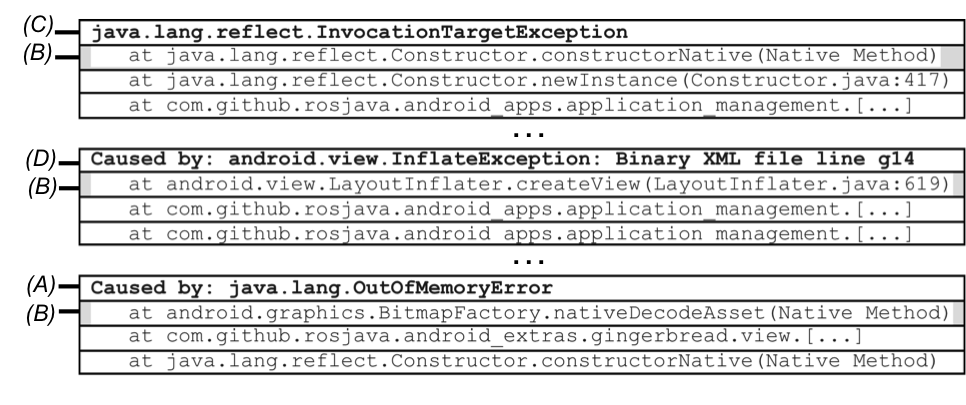
\includegraphics[scale=0.55]{stack_review6.png}
\caption{Example of an exception stack trace in Java.}
\label{fig:wrapping}
\end{figure}

\subsection{Best Practices}
\label{sec:best}

Several general guidelines have been proposed on how to use Java
exceptions~\cite{mandrioli1992advances,gosling2000java,wirfs2006toward,
bloch2008effective}. Such guidelines do not
advocate any specific exception type, but rather propose ways to effectively use each of them.
Based on these, for the purpose of our analysis we compiled the following list of Java exception handling best practices.

%\noindent\emph{Meaning of Exception Types}

\emph{I-Checked exceptions should be used to represent recoverable
conditions} (\cite{mandrioli1992advances,gosling2000java,wirfs2006toward,bloch2008effective}).
The developer should use checked exceptions for conditions from which the caller
is expected to recover. By confronting the API user with a checked exception,
the API designer is forcing the client to handle the exceptional condition. The
client can explicitly ignore the exception (swallowing, or converting it to
another type) at the expense of the program's robustness~\cite{gosling2000java}.

\emph{II-Error represents an unrecoverable condition which should not be handled} 
(\cite{gosling2000java}).  Errors should result from failures detected
by the runtime environment which indicate resource deficiencies, invariant
failures or other conditions, from which the program cannot possibly recover.

%\noindent\emph{Exception Throwing}

\emph{III-A method should throw exceptions that precisely define the
exceptional condition} (\cite{gosling2000java,bloch2008effective}). To do so,
developers should either try to reuse the exception types already defined in the
Java API or they should create a specific exception. Thus, throwing general types such as a
pure java.lang.Exception or a java.lang.RuntimeException is considered bad practice.

%\noindent\emph{Exception Documentation}
%\textbf{IV- It is wise to document all exceptions thrown by a method} 

\emph{IV- All exceptions explicitly thrown by reusable code should be documented.}
(\cite{mandrioli1992advances,gosling2000java,wirfs2006toward,bloch2008effective}).
For checked exceptions, this is automatically the case.
Bloch~\cite{bloch2008effective} furthermore recommends to document explicitly thrown
run time exceptions, either using a throws declaration in the signature, or using
the @throws tag in the Javadoc.
Doing so, in particular for public APIs of libraries or frameworks,
makes clients aware of all exceptions possibly thrown,
enabling them to design the code to deal with them and use the API effectively~\cite{Robil00,wirfs2006toward}.

%%%%%%%%%%%%%%%%%%%

\section{The Repository Mining Study}
\label{sec:study}

\begin{figure*} 
\centering 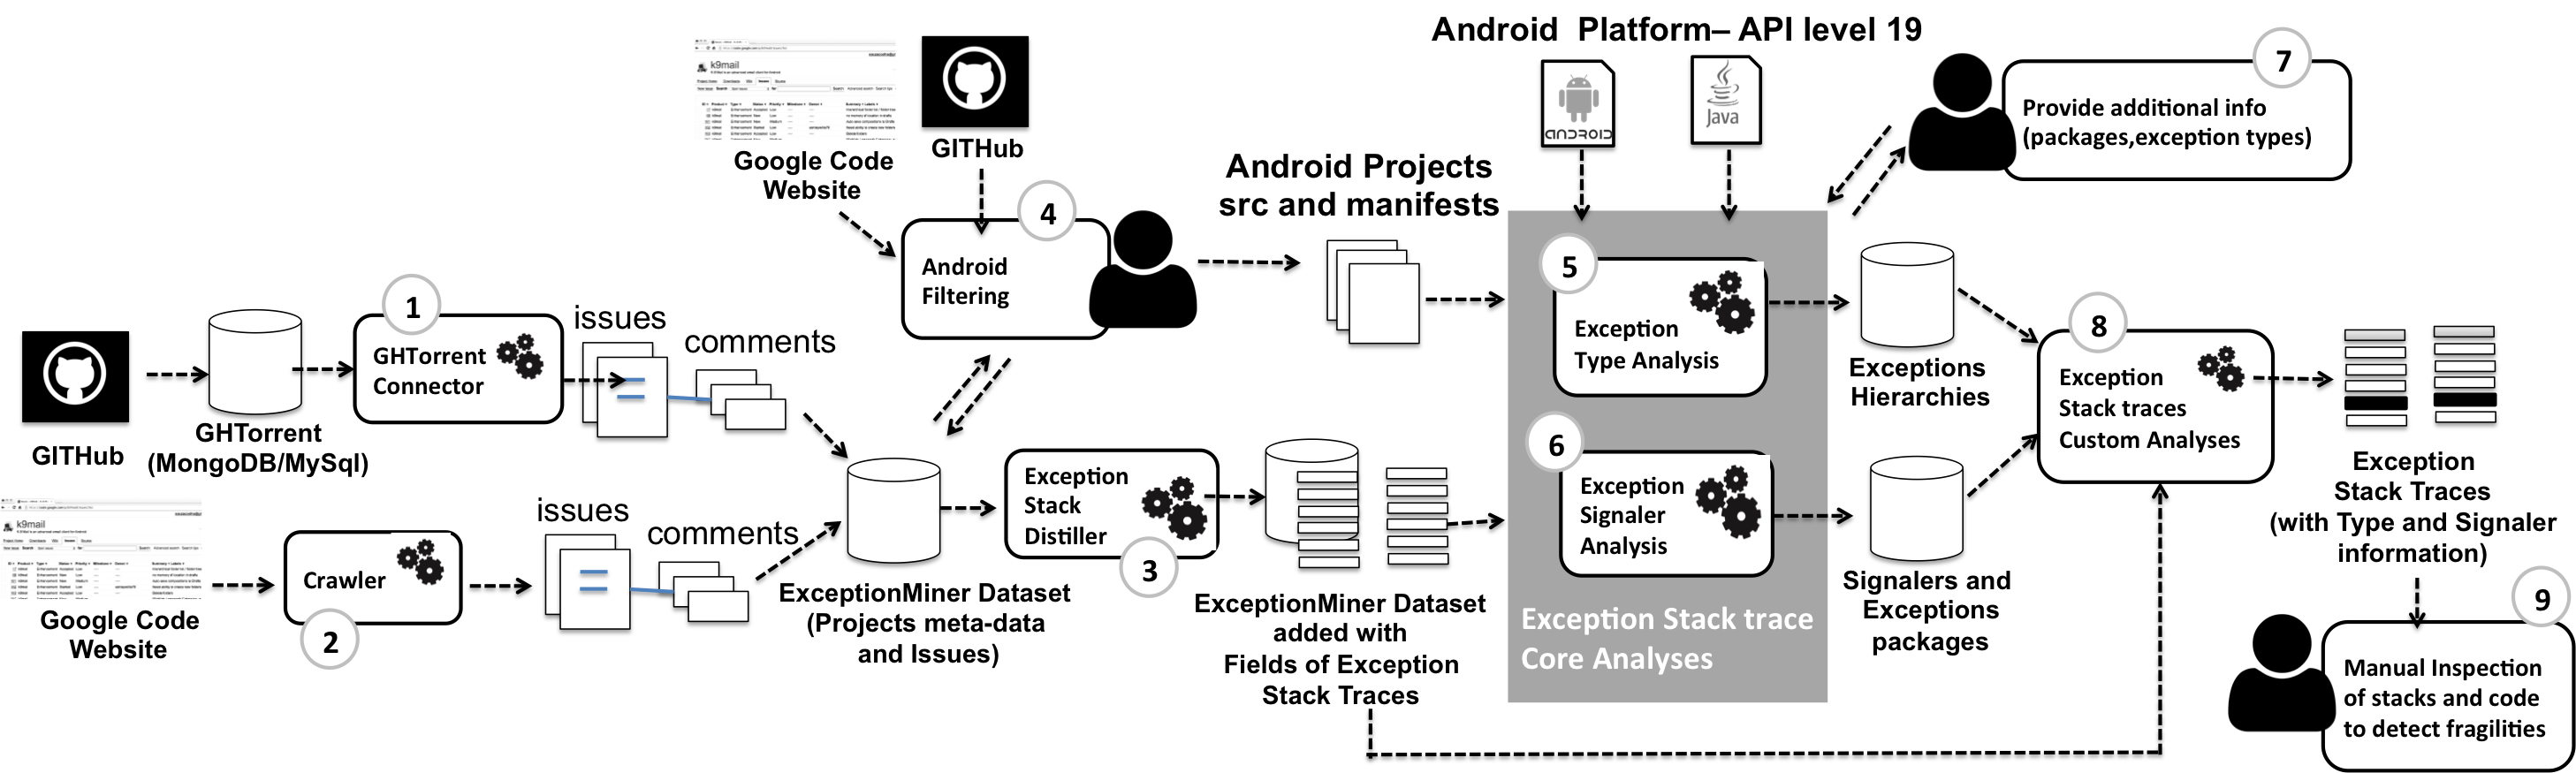
\includegraphics[width=.9\hsize]{overview_review.png}
\caption{Study overview.}\label{fig:overview} 
\end{figure*}

%This section describes the exploratory study whose goal was to investigate:
%\begin{description}
 % \item[RQ] \noindent\emph{Which fragilities on the exception-related code can be revealed from a post morten exception stack trace analysis of Android projects?} 
 %    \item
%\end{description}
%One major decision that had to be made for our investigation was the selection of the target 
%projects. We have selected a set of XXX open-source Android projects hosted in GitHub and 
%Google Code. GitHub and Google Code are among the most used hosting sites for open-source
 %projects,
% We investigate whether characteristics 
%of exception stack traces can pinpoint best practices violations and therefore reveal \emph{bug hazards}.

The goal of our mining study is to explore to what extent exception stack traces 
contained in issues of Android projects (hosted in GitHub and Google Code), can reveal 
\emph{bug hazards} in the exception-related code of both the applications and the underlying framework. 
As mentioned before, in this context \emph{bug hazards} are the characteristics of exception-related code 
that favor the introduction of failures such as uncaught exceptions. 
To support our investigation, we developed a tool called ExceptionMiner (Section~\ref{sec:exceptionminer})
which extracts the exception stack traces embedded on issues, 
and combines stack trace information with source code and bytecode 
analysis. Moreover, we use manual inspection to augment
 the understanding of stack traces and support further discussions and insights (Section~\ref{sec:manual}).
In this study we explore the domain quantitatively and highlight interesting cases by 
exploring cases qualitatively. 


Figure~\ref{fig:overview} gives an overview of our study.
First,  the issues reported on Android projects hosted on GitHub (1) and Google Code (2) are recovered.
Then the stack traces embedded in each issue are extracted and distilled (3).
The stack trace information is then combined with source code and bytecode analysis in order to discover 
the type of the exceptions (5) reported on the stack traces (e.g., error, runtime, checked),
and the origin (6) of such exceptions 
(e.g., the application, a library, the Android platform). 
Manual inspection steps (4, 7, 9) are used to support the mining process  and 
the search for \emph{bug hazards}  (8). The next sections detail each step of this mining process.

Our study focuses on open-source apps, since the information needed to perform our study
cannot be retrieved from commercial apps, whose issue report systems and 
source codes are generally not publicly available. 
Open source Android open-source apps have also been the 
target of other research~\cite{Linar13,Ruiz12} addressing the \emph{reuse} and API stability. 

%\subsection{Data Extraction Process}
%\label{sec:miningproc}

%In this exploratory study the following information is needed: (i) the issues reported on Android projects hosted on 
%GitHub and Google Code; (ii) the stack traces embedded on these issues; (iii) the type of the exceptions
 %reported on the stack traces (e.g., error, runtime, checked); (iv) the origin of such exceptions 
%(e.g., the application, a library, the Android platform). Next, we describe: how such information 
%was retrieved from GitHub and Google Code.

%mentioned 
%The data used in our study to answer our research questions are: the issues related to each 
%Android project available in each repository; the source code and manifest file of each application;
%the bytecode of all exceptions defined and reused by Android platform.


\subsection{Android Apps in GitHub}
\label{sec:git}


\begin{table}
  \scriptsize
  \centering
  \begin{tabular}{lr|lr}
    \hline
     \multicolumn{2}{c}{\bfseries{GitHub}} &  \multicolumn{2}{c}{\bfseries{Google Code}} \\
      \bfseries{Lable} &  \bfseries{\% Occurrences} &  \bfseries{Lable} &  \bfseries{\% Occurrences} \\
    \hline
empty &	54.24\% & Defect &	91.96\% \\
Defect &	39.56\%  & Enhancement  &	3.16\% \\
Enhancement &	0.57\% & Task	& 1.37\% \\
Support &	0.52\% & empty &	1.12\% \\
Problem &	0.36\% & StackTrace &	0.70\% \\
Others &	4.74\% &  Others &	1.68\% \\   
  \hline
  \end{tabular}
  \caption{Labels on issues including exception stack traces.}
  \label{tab:lables}
\end{table}

%As mentioned before, this study mined information available on GitHub issues,
%more specifically, extracting and distilling the stack traces embedded on GItHub issues. 

This study uses the dataset provided by the GHTorrent project~\cite{Gousi13}, 
an off-line mirror of the data  offered through the Github API.  
To identify Android projects, we performed a case insensitive search for the
term ``android" in the repository's names and short descriptions.  
Up to 23 February 2014,  when we queried GHTorrent, this resulted in 2,542 repositories. Running the ExceptionMiner tool 
 in this set we observed that 589 projects had at least one issue containing a stack trace.
	
Then we performed a further clean up, inspecting the site of every Android project
reporting at least one stack trace, to make sure that they represented real
mobile apps. During this clean up 107 apps were removed because they were either
example projects (i.e., toy projects) or tools to support Android development
(e.g. Selendroid, Roboeletric - tools to support the testing of Android apps).
The filtered set consisted of 482 apps. This set of 482 projects contained overall 31,592 issues from which 4,042 exception stack traces 
were extracted. 

Issues on Github are different from issues on dedicated bug tracking tools such as 
Bugzilla and Jira. The most important difference is that there are no predefined fields
  (e.g. severity and priority). Instead, Github uses a more open ended tagging system, on which
repositories are offered a pre-defined set of labels, but repository owners can modify 
them at will. Therefore, an issue may have none or an arbitrary set of labels depending 
on its repository. Table~\ref{tab:lables} illustrates the ocurrences of different labels 
on the issues including exception stack traces. Regardless of the issue labels, every exception stack
trace may contain relevant information concerning the exception structure of the
projects analyzed, and therefore can reveal \emph{bug hazards} on the exception-related code.
Because of this, we opted for not restricting the analysis to just defect issues.

%\footnote{We conducted the same analysis 
%on the defect issues only and the top exceptions were quite similar.
% Due to space limitation we limit to present the general analysis here. More detailed analysis
%on the defect issues can be found at:https://github.com/souzacoelho/exceptionminer}. 

\subsection{Android Apps in Google Code}
Google Code contains widely used open-source Android apps (e.g. K9Mail\footnote{K9Mail moved to Github but as a way of not loosing the project history it advises their users to report bugs on the Google Code issue tracker: https://github.com/k9mail/k-9/wiki/LoggingErrors.}).
However, differently from GitHub, Google Code does not provide an API to access the information related
 to hosted projects.\footnote{Google code used to provide a Web service to its repositories, but this was deactivated in June 2013 in what Google called a ``clean-up action''.}
To overcome this limitation we needed to implement a Web Crawler (incorporated in ExceptionMiner tool described next) that navigates 
through the web interface of Google Code projects extracting all issues and issue comments and storing them in a relational database for later analysis.
To identify Android projects in Google Code, we performed a similar heuristic: we performed a case insensitive search 
(on the Google Code search interface) for the term ``android''. On January 2014, when we queried Google Code, this resulted in a list of 788  projects. This list comprised the seeds sent to our Crawler.

The Crawler retrieved all issues and comments for these projects.
From this set, 724 projects defined at least 1 issue. Running the ExceptionMiner tool 
 in this set we observed that 183 projects had at least one issue containing an exception stack trace.
 Then we performed further clean up (similar to the one described previously) inspecting the site 
of each project. As a result we could identify 157 Android projects.  This set contained  127,456 issues in total,
 from which 1,963 exception stack traces were extracted. Table~\ref{txab:lables} illustrates the occurrences of different labels 
on the issues including exception stack traces. Differently from GitHub, in Google Code most of 
the issues were labeled as ``Defect''. However, based on the same assumption described for the GitHub repository
 we considered all issues reporting stack traces (regardless its labels).

%SELECT distinct(type), count(*) as n
%  FROM exceptionalissue where repo !='android' group by type order by n desc;

%For instance: K9mail  was hosted in Google Code 
%before moving to GitHub and in order not to loose the project history it advices their 
%users to create issues on Google Code as a way to preserve project history.

%To overcome this limitation and mine the information available on such Google Code 
%projects we implemented a Web crawler which navigated (incorporated in ExceptionMiner tool described next) 
% on each project and issue page, extracting the content of each issue to store on relational database.

%{MOSTRAR UMA FIGURA COM TODOS OS PASSOS E RESSALTAR OS PASSOS MANUAIS}
%COMPLETE HERE.....
%\subsubsection{Database of Exception Stack Trace Information}
%\subsubsection{Distiling Exception Stack Trace Information}
%\subsection{Process}
%ESPALHAR ESTA SECAO NAS OUTRAS.
%Figure~\ref{fig:overviewfig} presents an overview of the mixed-methods approach
%conducted to answer these questions. The mixed-methods approach is composed by the following steps:

\subsection{The ExceptionMiner Tool}
\label{sec:exceptionminer}

The ExceptionMiner is a tool which can connect to different issue repositories, 
extract issues, mine exception stack traces from them, distill exception stack trace information,
and enable the execution of different analyses by combining exception stack 
trace information with byte code and source code analysis. The main components of ExceptionMiner are the following:

\emph{\textbf{Repository Connectors.}} This component enables the connection 
with issue repositories. In this study two main connectors were created: one which connects to 
GHTorrent database, and a Google Code connector which is comprised of a Web Crawler
 that can traverse the Google Code web interface and extract the project's issues. 
Project meta-data and the issues associated with each project are stored in a relational 
database.

\emph{\textbf{Exception Stack Trace Distiller.}}
This component combines a parser (based on regular expressions) 
and heuristics able to identify and filter exception names and stack traces inline with text. 
This component distills the information that composes a stack trace.
 Some of the attributes extracted from the stack trace are
 the root exception and its signaler, as well as the exception wrappers and their corresponding signalers. 
This component also distills fine grained information of each attribute such as the classes and packages associated to them.
In contrast to existing issue parsing solutions such as Infozilla, our parser
 can discover stack traces mixed with log file information\footnote{In several 
exception stack traces, the exception frames were preceeded by logging information e.g., 
\texttt{03-01 15:55:01.609 (7924): at android.app.ActivityThread.access\$600(ActivityThread\-.java:127)} which could not be detected by existing tools.}.

\emph{\textbf{Exception Type Analysis.}} To support a deeper investigation of the 
stack traces every exception defined on a stack trace needs to be classified according to its type
(e.g. Error, checked Exception or RuntimeException). The module responsible for this analysis 
uses the Design Wizard framework \cite{Brunet09} to inspect the bytecode of the exceptions reported 
on stack traces.  It walks up the type hierarchy of a Java exception until it reaches 
a base exception type. Hence in this study the bytecode analysis was used to discover the type 
of each mined exception when the jar file of such exception was available on the project or 
on a reused  Java library. A specific implementation (based on source code analysis)
 was needed to discover the exception type when the bytecode was not available.
With this module we analyzed all exceptions defined in the Android platform (Version 4.4, API level 19),
which includes all basic Java exceptions that can be thrown during the app execution,
and exceptions thrown by Android core libraries. Moreover, we also analyzed the 
exceptions reported on stack traces that were defined on applications and third-party libraries 
(the tool only analyzed the last version available).

\emph{\textbf{Exception Signaler Analysis.}}
This module is responsible for classifying each signaler according 
to its origin (i.e., Android Application Framework, Android Libcore, Application, Library). 
Table~\ref{tab:signalers} presents the heuristics adopted in this classification.
To conduct this classification, we provide this module with the information
comprising all Java packages that compose: the Android Plaform;
 the Android Libcore; and each analyzed Application. To discover the packages for the first two origins
we can use the Android specification.
To discover the packages for the third origin, the application itself, this module
extracts the manifest files of each Android app, which defines the main packages that the applications consist of.
 If this file is not available, the tool recursively analyzes the 
structure of source-code directories composing the appm filtering out the cases in which the application also includes the source code of reused libraries.
Then, based on this information and using pattern matching 
between the signaler name and the packages, this module identifies 
the origin of the exception signalers. 

The exceptions are considered to come
 from libraries if their packages are neither defined 
within the Android platform, nor on core libraries, nor on applications.
Table~\ref{tab:signalers} summarizes this signaler classification.

%\noindent\emph{Exception Wrapping Analysis.} 
%\noindent\emph{Concern Mapping.} 

\begin{table}
  \centering
  \scriptsize
  \begin{tabular}{rp{29em}}
    \hline
    \bfseries{Signaler} & \bfseries{Description} \\
    \hline
    \bfseries{android} & If the exception is thrown in a method defined in Android platform.\\
    \bfseries{app}     & If the exception is thrown in an method defined on an Android app.\\
    \bfseries{libcore} & If the exception is thrown in one of the core libraries reused by Android (e.g., org.apache.harmony, org.w3c.dom, sun.misc, org.apache.http, org.json, org.xml). \\
    \bfseries{lib}     & If the exception is thrown on a method that was not defined by any of the elements above.\\
    \hline
  \end{tabular}
  \caption{Sources of exceptions in Android}
  \label{tab:signalers}
\end{table}

\subsection{Manual Inspections}
\label{sec:manual}
In our experiments, the output of the ExceptionMiner tool was manually extended
in order to 
(i) support the identification of packages composing the Android platform, 
libs and apps analyzed in this study (as described previously); and (ii)  
identify the type of some exceptions reported in issues 
that were not automatically identified by the ExceptionMiner tool
(because they were defined on previous versions of libraries,
apps and Android Platform). When the exception could not be  
found automatically or manually (because they were defined on a previous version
of the app or lib), we classified the exception as ``Undefined''.  Only 31 exceptions 
remained undefined, which occurred in 60 different exception stack traces (see Table~\ref{tab:typeroottab}).

\subsection{The Mining Study Results}
\label{sec:result}

%This section presents the results of the study, providing both a
%quantitative and qualitative analysis of the outcomes. 
%We center our presentation of the results around \emph{bug hazards} we
%distilled from (1) common root exceptions; (2) exception types; and
%(3) exception wrappings.

This section presents the results of the study; this presentation is centered around 
the information distilled from stack traces: (i) the root exceptions (i.e., the exceptions that caused the stack traces);
 (ii) the exception types (i.e, Checked, Runtime, Error, Throwable) and (iii) the exception wrappings. 
Each piece information is then analyzed in detail to 
check whether they can reveal bug harzards on the exception handling code -
related to (i) specific violations of the best practices presented in Section~\ref{sec:best},
or (ii) the general use of exception handling to suport robust development.

\subsubsection{Can the root exceptions reveal bug harzards?}
After distilling the information available on the exception stack traces, we could find 
the exceptions commonly reported as the root causes of stack traces.
Table \ref{tab:topten} presents a list of the top 10 root exceptions found in the study - 
 ranked by the number of distinct projects on which they were reported. 
This table also shows how many times the signaler of such an exception was a method defined on
the Android platform, the Android libcore, the application itself or a third-party library -
 following the classification presented in Table  \ref{tab:signalers}. 

\begin{table*}
  \tiny
  \centering
%  \begin{tabular}{rcccccccc}
  \begin{tabular}{lrrrrrrrr}
    \hline
    \bfseries{Root Exception} &  \multicolumn{2}{c}{\bfseries{Projects}} &  \multicolumn{2}{c}{\bfseries{Occurrences}} & \textsf{Android} & \textsf{Libcore} & \textsf{App} & \textsf{Lib} \\
    & \bfseries{\#} &  \bfseries{\%} & \bfseries{\# } & \bfseries{\% } &&&&\\
    \hline

java.lang.NullPointerException	&	332	&	51.96\%	&	1664	&	27.71\%	&	525	&	20	&	836	&	280	\\
java.lang.IllegalStateException	&	120	&	18.78\%	&	278	&	4.63\%	&	185	&	31	&	41	&	39	\\
java.lang.IllegalArgumentException	&	142	&	22.22\%	&	353	&	5.88\%	&	195	&	12	&	95	&	44	\\
java.lang.RuntimeException	&	122	&	19.09\%	&	319	&	5.31\%	&	203	&	2	&	64	&	51	\\
java.lang.OutOfMemoryError	&	78	&	12.21\%	&	237	&	3.95\%	&	141	&	16	&	35	&	34	\\
java.lang.NoClassDefFoundError	&	67	&	10.49\%	&	94	&	1.57\%	&	10	&	0	&	46	&	37	\\
java.lang.ClassCastException	&	64	&	10.02\%	&	130	&	2.16\%	&	55	&	0	&	55	&	20	\\
java.lang.IndexOutOfBoundsException	&	62	&	9.70\%	&	166	&	2.76\%	&	53	&	0	&	93	&	18	\\
java.lang.NoSuchMethodError	&	54	&	8.45\%	&	80	&	1.33\%	&	10	&	0	&	56	&	14	\\
java.util.ConcurrentModificationException	&	43	&	6.73\%	&	65	&	1.08\%	&	5	&	0	&	46	&	13	\\
    \hline
  \end{tabular}
\caption{Root Exceptions occurrences and popularity in repositories hosted in Google Code (GC) and GitHub(GH).}
\label{tab:topten}
\end{table*}
 
We can observe that most of the exceptions in this list are implicitly thrown by the
 runtime environment due to programming mistakes  (e.g., out-of-bounds array index, division-by-zero, access to a null reference)
 or resource limitations (e.g., OutOfMemoryError). 
From this set the java.lang.NullPointerException was the most reported root cause (27.71\%). 
If we consider the frequency of NullPointerException 
across projects, we can observe that 51.96\% of all projects reported at least one exception stack 
trace on which the NullPoiterException was the root cause.

 The NullPointerException was mainly signaled inside the application code (50\%) and the Android platform (31.5\%),
 although we could also find the NullPointerException being signaled by third-party libraries (16.3\%). 
Regarding reusable code (e.g., libraries and frameworks), there is no consensus whether it is a good or a bad practice to 
explicitly throw a NullPointerException. Some prefer to encapsulate such an exception on
an instance of IllegalArgumentException, while others~\cite{bloch2008effective} argue that the
NullPointerException makes the cause of the problem explicit and hence 
can be signalled by an API expecting a non-null argument.The high prevalence of NullPointerException is aligned with the
findings of other 
research~\cite{kim2013predicting,fraser20131600,csallner2004jcrasher,kechagia2014}. 
For instance, Kechagia and Spinellis showed that the NullPointerException was the  
most reported exception on the crash reports sent to BugSense (a bug report 
management service for Android applications)  \cite{kechagia2014}.
Other research on robustness testing~\cite{maji2012empirical,csallner2004jcrasher} shows that most of the automatically 
detected bugs were due to NullPointerException and exceptions
implicitly-signaled by the Java 
environment due to programming mistakes or resource limitations
 (as the ones found in our study).

%Sunghun et
%al.~\cite{kim2013predicting} show that 38\% the bugs related to
%exception handling in the Eclipse project
%are caused by NullPointerException.
%Furhtermore, 

\emph{\textbf{Identifying the Concerns Related to Root Exceptions.}} To get a broader view of the root exceptions of stack traces,
we performed a manual inspection in order to identify the underlying
concerns related to the most frequently reported root exceptions.
Besides the exceptions related to programming mistakes mentioned before, we also looked for exceptions related to some concerns that are known as sources of faults in mobile development: concurrency~\cite{ama2012} backward compatibility~\cite{McDon13}, security~\cite{enck2011study,was2010} and resource management (IO, Memory, Batery)~\cite{Zhang12}. Since it is infeasible to inspect the code responsible for throwning every exception reported in this study,
the concern identification of each exception was based on intended
meaning of the particular exception type, as defined in 
its Javadoc documentaion and in the Java specification. 
For example: (i) an instance of ArrayOutOfBoundException  
refers to a programming mistake according to its Javadoc; and (ii) the Java specification lists all 
exceptions related to backward compatibility~\cite{javaback}, such as
InstantiationError, VerifyError, and IllegalAccessError.

To perform this concern analysis, we selected a subset of all reported
root exceptions, consisting of 100 exceptions
reported in 95\% of all stack traces analyzed in this study. Hence, based on the inspection of the 
Javadoc related to each exception and the Java specification, we
identified the underlying concern releated to each root exception. 
Table~\ref{tab:tophundrend} contains the results of this analysis. This table also illustrates the exceptions 
that could not be directly mapped to one of the aforementioned concerns, either because they were too general (i.e., java.lang.Exception,
java.lang.RuntimeException, java.lang.Error) or because they were
related to other concerns (e.g., specific to an application or a given library). 
To ensure the quality of the process, three independent coders classified a randomly selected
sample of 25 exception types (from the total 100) using the same list of concerns;
the inter-rater agreement was 96\%.

\begin{table}
\scriptsize
\centering
\begin{tabular}{lrr}
\hline
\bfseries{Concern} & \bfseries{\% Occurrences on stacks} \\
\hline
Programming logic (java.lang and util) & 52,0\%\\
Resources (IO, Memory, Batery) & 23,9\% \\
Security & 4,1\%\\
Concurrency & 2,9\% \\
Backward compatibility & 5,5\% \\
Specific Exceptions & 4,9\%\\
General (Error, Exception, Runtime) & 6,7\%\\
\hline
\end{tabular}
\caption{Identifying the concerns related to root exceptions}
\label{tab:tophundrend}
\end{table}

This analysis revealed that approximately 75\% of the exceptions
 that caused the stack traces are implicitly thrown by runtime 
environment  due to mistakes on programming logic (e.g., out-of-bounds array index, null pointer 
references) and resource limitations. Although such exceptions do not directly point to violations on
the best practices described before (which are related to the 
explicitly thrown exceptions) they impose a major threat to apps robustness,
and therefore represent a critical bug hazard to the exception 
handling code of Android applications. 
Security and concurrency, which are known to be critica issues on  Android apps, 
raised few of the reported exceptions (less then 5\% of the anlysed stack traces).

%\finding{%
%More than 50\% of the uncaught exceptions analyzed in this study are due to errors in
%programming logic, with the NullPointerException as most prevalent
%exception.
%For another 25\% the root cause relates to resource constraints.
%}

\bigskip 

\finding{%
Exceptions related to programming logic and resource limitations represent a major bug hazard to Android apps - 
since they represent approximately 75\% of the exceptions that caused the stack traces.
From this set the NullPointerException as most prevalent exception.
}

\subsubsection{Can the exception types reveal bug hazards?}
%\subsection{Exploring the Information Embedded on Exception Types}
%\subsection{The Exception Types and What They can Tell us? }

As mentioned before, using the ExceptionMiner tool in combination with manual inspections we could identify
the root exception \emph{type} (i.e., RuntimeException, Error, checked Exception) as well as its \emph{origin} - which we 
identified based on the package names of the signalers related to it in the stack traces (Section~\ref{sec:exceptionminer}).
Table~\ref{tab:typeroottab} presents the types and origins of root exceptions of all analyzed stack traces. 

We can observe that most of the reported exceptions are of type runtime 
(64.85\%); and that the most common origins are methods defined either on the Application (47.3\%)
or on the Android platform (34.3\%). We could also find runtime exceptions thrown by library code (17.7\%).
 We can also see, from Table~\ref{tab:typeroottab}, that in contrast with the other origins, most of the 
 exceptions signaled on Android Libcore (i.e., the set of libraries reused by Android) are 
checked exceptions. This set comprises: org.apache.harmony, org.w3c.dom, sun.misc, 
org.apache.http, org.json, org.xml, and javax. Signaling checked exceptions is considered a 
good practice (see best practice IV in Section~\ref{sec:best}) because by using 
checked exceptions a library can define a precise 
\emph{exception interface}~\cite{miller1997issues} to its clients.
 Since such libraries are widely used  in several projects, this
 finding can be attributed to the libraries' maturity.

%SELECT COUNT(*) FROM STACKTRACESUMMARY WHERE
% repo !='android'  AND MAIN_EXTENDS LIKE 'RUNTIME%' 
%SELECT COUNT(*) FROM STACKTRACESUMMARY WHERE
%repo !='android'  AND MAIN_EXTENDS LIKE 'RUNT%' AND MAINSIGNALER_FROM like 'APP%';

\begin{table}
\scriptsize
\centering
\begin{tabular}{lrrrrrr}
    \hline
    \bfseries{Root Type} & \bfseries{Android} & \bfseries{Libcore} & \bfseries{App} & \bfseries{Lib}  & \bfseries{All} & \bfseries{\%} \\
    \hline

Runtime	&	1335	&	73	&	1843	&	690  &	3894 & 64.85\% \\  %2466+854
Error	       &	 188              &	 46	&	302             &	167	           &	691 & 11.51\%	\\
Checked	&	276           &	314	&	313          &	567	           &	1358 & 22.61\%	\\
Throwable	&	0	       &	0	&	2            &	0         &	2 & 0.03\%	\\
Undefined	&	4	&	0	&	18		&	38	   &	60	& 1.00\% \\
 \hline
All		& 1  803	&	433	&	2478	&	1462	&	6005 	\\
    \hline
  \end{tabular}
\caption{Types and origins of root exceptions.}
  \label{tab:typeroottab}
\end{table}

\bigskip

\finding{Almost two thirds of all crashes come from runtime
  exceptions. Most of these originate from the application layer.}

\bigskip

\emph{\textbf{Inspecting Exception Interfaces.}}  According to the best practices mentioned before, 
 \emph{explicitly thrown} runtime exceptions 
should be documented as part of the \emph{exception interface} of libraries/framework reusable
methods. To investigate the conformance to this practice, we firstly filtered out all the exceptions implicitly
 signaled by  the runtime environment (due to programming mistakes) - since these exceptions 
should not be documented on the method signature.  Then we inspected
the code for each method 
(defined either in the Android  Aplication Framework or in third-party libraries) 
explicitly signaling a runtime exception. 
Table~\ref{tab:runtimeinterface} presents the results of this inspection. 
We found 79 methods (both from libraries and the Android platform) that  explicitly threw a runtime exception 
without listing it on the \emph{exception interface} (i.e., using 
throws clause in the method signature). From this set only one method (defined on a library)
included an @throws tag in its Javadoc - reporting that the given runtime exception
could be thrown in some conditions. These methods were responsible for 
267 exception stack traces mined in this study.

This result is in line with the results of two other studies~\cite{sacramento2006unchecked,kechagia2014}. 
Sacramento et al~\cite{sacramento2006unchecked} observed that the
runtime exceptions in .NET programs are most often not documented. 
Kechagia and Spinellis~\cite{kechagia2014} identified a set of methods 
on the Android API which do not document its runtime exceptions. One limitation 
of the latter work is that it did not filter out exceptions that,  
although runtime, should not be documented because they were implicitly signaled by the 
JVM due to resource restrictions or violations on Java semantic constraints.
When explicitly signaling a runtime exception and not documenting it, 
the developer imposes a threat to system robustness, especially
when such exceptions are thrown by third party code (e.g., libraries or framework utility code)
 invoked inside the application. In such cases the developer usually does not have access to 
the source code. Hence in the absence of the exception documentation it is very difficult or even impossible
 for the client to design the application to deal with ``unforeseen'' runtime exceptions. As a consequence, the
 undocumented runtime exception may remain uncaught and lead to system crashes.

\bigskip

\finding{%
Only a small fraction (4\%, 267 stack traces) of runtime exceptions are programmatically
thrown. Almost none (0.4\%, just one) of these were documented. Such undocumented 
runtime exceptions violate best practices III and IV reveal a bug harzard to Java/Android apps.}

\bigskip

\begin{table}
\scriptsize
\centering

 %\begin{tabular}{|p{7.9cm} p{0.1cm}|}
\begin{tabular}{lrrrr}
    \hline
 \bfseries{Origin}   &  \bfseries{stacks}  & \bfseries{signaler methods} &  \bfseries{throws clause}  &  \bfseries{@throws}  \\ 
\hline					
Libraries	& 	205	 & 	44	& 0	& 1	\\
Android  	&	62 &	35	&0 &  0	\\					
\hline					
\bfseries{All}	&	267 &	79 &  0  & 1\\
\hline					
  \end{tabular}
\caption{Absence of exception interfaces on methods.}
\label{tab:runtimeinterface}
\end{table}

\emph{\textbf{Missing Checked Exceptions on Exception Interfaces.}} 
Our exception stack trace analysis revealed an unexpected bug hazard: a 
checked exception thrown by a native method and not declared on the exception 
interface of these methods signaling them. The native method in question was defined in
 the Android platform, which uses Java Native Invocation (JNI) to access 
native C/C++ code. This exception was thrown by the method getDeclaredMethods defined in java.lang.Class. 
The Java-side declaration of this method does not have any throws clause, 
leading programmers and the compiler to think that no checked exceptions can be thrown.
 However, the C-code implementation did throw a ``checked exception" called NoSuchMethodException, 
violating the declaration. The Java compiler could not detect this violation, because it does 
not perform static exception checking on native methods. This type of bug is hard to diagnose
because the developer usually does not have access to the native implementations. 
Consequently, since it is not expected by the programmer, when such a method throws 
this exception, such an undocumented exception may remain
uncaught and cause the app to crash, or maybe mistakenly handled by subsumption.
The exception stack traces reporting this scenario actually correspond
to a real bug of Android 
Gingerbread version (which still accounts for 13.6\% of devices running Android).
%Among the Android projects on which this exception stack trace was reported we can cite:
%PageTurner (206 stars), ActionBarSherlock (6,041 stars), otto (1,618
%stars).

\bigskip

\finding{%
For native methods, even checked exceptions can be
thrown without being documented on the exception interface.
It violates best practices III and IV and represent a bug hazard
 hard to diagnose.
}

\bigskip

\subsubsection{Can the exception wrappings reveal bug hazards?}


\begin{table}
\scriptsize
\centering

 %\begin{tabular}{|p{7.9cm} p{0.1cm}|}
\begin{tabular}{ll}
    \hline
 id & \bfseries{Runtime Exception wrapping an Error}    \\  %\bfseries{\#}
    \hline
1 & java.lang.RuntimeException - java.lang.OutOfMemoryError  \\ %30
2& java.lang.RuntimeException -  java.lang.StackOverflowError)   \\ %4
\hline
& \bfseries{Checked Exception wrapping an Error}  \\
 \hline
3&java.lang.reflect.InvocationTargetException - java.lang.OutOfMemoryError  \\ %5
4&java.lang.Exception - java.lang.OutOfMemoryError   \\ %1
\hline
& \bfseries{Error wrapping a Checked Exception}  \\
 \hline
5&java.lang.NoClassDefFoundError - java.lang.ClassNotFoundException   \\ %4
6&java.lang.AssertionError - javax.crypto.ShortBufferException)   \\ %3
\hline
& \bfseries{Error wrapping a Runtime Exceptino}    \\
 \hline
7&java.lang.ExceptionInInitializerError - java.lang.NullPointerException   \\ %9
8&java.lang.ExceptionInInitializerError - java.lang.IllegalArgumentException 	 \\ %2
 \hline
  \end{tabular}
\caption{Examples of Cross-type wrappings}
\label{tab:exampeswrap}
\end{table}


\begin{table*}
\scriptsize
  \centering
  \begin{tabular}{llcccccc}
    \hline
    \bfseries{Wrapper}  &  \bfseries{Root Cause} &  \bfseries{Projects}  &  \bfseries{Occurrences} & \textsf{Android} & \textsf{Java/Libcore} & \textsf{Lib} & \textsf{App}  \\
    \hline
      
      Runtime &  Checked   & 88 & 148 &  75 &  0   & 38 &  35 \\  %(50.7\%) 
      Runtime   &  Error      & 46  &  67    &  58  &  0   & 8  &  1   \\      %(86.5\%) 
      Checked &  Runtime   & 17  & 31 & 4 &  0  & 16  &  11 \\  %(51.6\%) 
      Checked & Error         & 8    &  9  & 5  &  0  &  1 &  3  \\
      Error & Checked         & 14  &  27 &  6  &  7  &  6 &   8    \\
      Error & Runtime        & 8      &  17   & 1 &  1  & 1 &  14    \\

  \hline
      %none   & Runtime   &  2360 & 359 \\
      %none  &   Checked  & 422  & 117 \\
      %none  &   Error   & 381  & 141 \\
      %none &  Undefined  &  15   & 10  \\
      %none & Throwable  &  1    & 1 \\
     %\hline
      %Runtime   & Runtime & 560  & 182 \\    
      %Checked   & Checked & 98   & 42  \\
      %Error     & Error   & 15   & 14  \\
    %\hline
  \end{tabular}
\caption{Wrappings comprising different exception types.}
\label{tab:wrappingandroid}
\end{table*}

Java is the only language that provides a hybrid exception model 
which offers three kinds of exceptions each one holding an intended exception behavior (i.e., error, 
runtime and checked). Table~\ref{tab:wrappingandroid} presents some wrappings found in this study that
include different exception types (i.e., Error, checked Exception and Runtime).
Below, we discuss the most
important of such ``cross-type wrappings in more detail.

\emph{\textbf{Runtime Exception wrapping an Error.}} 
From Table~\ref{tab:wrappingandroid}, we see that most of these wrappings	
are performed by the Android platform (50.7\%).
The code snippet below was extracted from Android and shows a general catch clause 
that converts any instance of Throwable (signaled during the execution
of an asynchronous task) into an instance of RuntimeException and re-throws it.  
Table~\ref{tab:exampeswrap} presents examples of exceptions that were actually wrapped in this code snipet.  
Such wrappings mask an unrecoverable Error into a general runtime exception.

%{\footnotesize
%\begin{verbatim}
%   try {
%      ...
%   } catch (InterruptedException e) {
%      android.util.Log.w(..., e);
%   } catch (ExecutionException e) {
%      throw new RuntimeException("...",e.getCause());
%   } catch (CancellationException e) {
%      ...
%   } catch (Throwable t) {
%     throw new RuntimeException("...", t);
%   }
%\end{verbatim}
%}


{\footnotesize
\begin{verbatim}
   try {
      ...
   } catch (InterruptedException e) {
      android.util.Log.w(..., e);
   } catch (ExecutionException e) {
      throw new RuntimeException("...",e.getCause());
   } catch (CancellationException e) {
      ...
   } catch (Throwable t) {
     throw new RuntimeException("...", t);
   }
\end{verbatim}
}

\emph{\textbf{Runtime Exception wrapping a Checked Exception.}} 
This wrapping was responsible for 49.5\% of
the cross-type wrappings.  From this set 50\%  were performed on methods defined on Android platform. 
We observe that it is a common implementation practice in the methods of Android platform.
However, using such a general exception, is considered a bad practice
according to the Java specification and common guidelines, as it loses contextual information about the exception.

\bigskip

\finding{%
General catch clauses masking any exception into a general RuntimeException 
is a common practice in the Android Platform; it violates best practice III 
and is considered a bug hazard as it loses contextual information about the exception.
}

\bigskip

\emph{\textbf{Checked Exception wrapping an Error.}} Most of these wrappings
 were also caused by the reflection library used by applications' methods. The methods responsible for the wrappings
were also native methods written in C. Table~\ref{tab:exampeswrap} illustrates
some of these wrappings some of them are masking an OutOfMemoryError
into a checked exception. Such wrappings may also mask an unrecoverable error
and may lead to ``exception confusion'' described next.

\emph{\textbf{Error wrapping Runtime and Checked Exceptions}} Table~\ref{tab:exampeswrap}  illustrates
examples of instances of Error wrapping instances of
RuntimeException. 
Although such a wapping mixes different exception types,
since there is no obligation associated to handling runtime exceptions, it
does not violate the aforementioned best practices. 

On the other hand, the inspection 
also revealed instances of Error wrapping checked exceptions. Such wrappings were 
mostly performed by Java static initializers. If any exception is thrown in the context of a static initializer 
(i.e., static block)  it is converted into an ExceptionInitializerError 
on the point where the class is first used.  Table~\ref{tab:exampeswrap} also illustrates
examples of such wrappings. Although such a wrapping may represent a design decision,
it violates the best practices related to checked exceptions and errors as it mixes the intended handling 
behaviour associated to both types.

We can also observe that some stack traces include successive cross-type wrappings, 
such as: Runtime - Checked - Runtime - Checked - Runtime - Checked -
Runtime. 
Hence, although some of these wrappings may be a result from design decisions, the mis-use of exception wrapppings may make the exception handling 
code more complex (e.g., the multiple wrappings) and error-prone,
 and lead to ``exception confusion''. To illustrate this problem we can use one of the wrappings discussed above.
When the developer is confronted with a checked exception, the designer of the API is telling him/her 
to handle the exceptional condition (according to Java Specification and 
best practices). However, such exception may be wrapping an Error such
as an OutOfMemoryError, which indicates a resource deficiency 
that the program cannot possibly recover from). Hence, trying to
handle such an exception  
may lead the program to an unpredictable state.

\bigskip

\finding{%
Cross-type exception wrappings are common.
They represent a bug hazard once they violate the semantics of Java's original exception
design, detailed on best practices I and II  (e.g., when mapping unrecoverable Errors to other types of
exceptions). 
}

\bigskip

\section{The Developers Perspective}
\label{sec:dev}

Although the mining study revelaed a set of bug hazards in Android exception handling no work had examined yet what are the developers perceives about them. With Android development rapidly rising in popularity, it is important to better understand how developers deal with such bug hazards and what they do to overcome them. 

To better understand the developers perspective about the bug hazards detected during the mining study, we set up an exploratory qualitative investigation and survey Android developers on how they face such bug hazards in their projects. Our field of study is GitHub; using our GHTorrent database~\cite{Gousi13}, we aimed our survey at developers from Android projects available in GitHub and which issues were mined during the first phase of this study. 

Our main goal is to learn from developers perspective about the Java exception handling usage and the main exception handling bug hazards in Android. We therefore use a survey as our main research instrument. The survey mixed  Liket-scale with open-ended questions. The questions were motivated by the analysis of the existing bug hazards detected in the first phase of this study. Next sections detail the survey.

%Our main findings reveal that developers often handle exceptions while developing Android apps and 
%we provide insights into the main challenges faced by them during this task. xxxxxxx


\subsection{Research Questions}

When developing Java-based applications it is inevitable to deal with exceptions. Consequently, our first question explores how developers deal with the exception handling code in Android development:

\emph{\textbf{RQ 1:} How often developers with the exception handling code while developing Android apps?} 

To make the analysis easier, we further refine RQ1 in subquestions, such as: \emph{How often developers handle exceptions?}; \emph{How often developers throw exceptions?}. Moreover, another question that show us how developers may deal with the EH code is: \emph{Do they knew about Java EH best practices and/or Android specific EH best practices?}
 
Then following research question focus on the developers perspectives about the main bug hazards found during the mining study, more specifically: 

\emph{\textbf{RQ 2:} How the NullPointerExceptions impact the development of robust Android apps?}

\emph{\textbf{RQ 3:} How cross-type wrappings impact the development of robust Android apps?}

\emph{\textbf{RQ 4:} Are developers aware of the robustness threats caused by JNI undocumented checked exceptions?}

%\emph{\textbf{RQ 4:}  Are developers aware of the non-declared checked exceptions?}


%\emph{RQ 2:Have developers ever faced a crash caused by NullPointerException?}
%\emph{RQ 3:Are developers aware of the robustness threats caused by cross-type wrappings?}; %\emph{RQ 4: Are developers aware of the robustness threats caused by JNI undocumented checked exceptions?}

Some of such questions were indirectly answered by presenting a set of code snippets on which
the bug hazards were present and asked developers what they would do when faced with such scenarios.

Finally developers were asked whether the exception handling code helped with the development of robust Android applications, and what they usually do to prevent apps from crashing. Hence, the last research question that guided this survey was the following:

\emph{\textbf{RQ 5:} How the exception handling code affect the development of robust apps and how developers prevent apps from crashing?}

\subsection{Protocol}

Since our aim is to learn from a large number of developers, we use surveys which scale well.
The survey is split into two logical sections; multiple choice or Likert-scale questions and open-ended questions. The multiple choice questions are intermixed with open-ended questions to further elicit the developer’s opinions. Moreover, the survey also contains Likert scales questions to force participants to make a choice. Overall, the survey includes 13 open-ended questions, 5 Likert scale questions and 10 multiple choice questions. The respondents could fill in the survey in about 15 minutes.

We used grounded theory coding~\cite{charmaz2006}, iterating through our open-ended survey responses, to answer some of the research questions. The grounded theory coding used in this study consists of at two phases: (1) initial coding entails a close reading of the data and (2) later we use focused coding ~\cite{charmaz2006} to pinpoint and develop the most salient themes~\cite{charmaz2006} in the analyzed data.

\subsection{Participants}

 In previous work~\cite{coelhoetal15}, we mined exception stack traces available on issues reported on several Android projects hosted in GitHub and Googlecode. To ensure that our sample consists of repositories that were real Android apps, we had to inspect every project site and discard the toy-programs and non-Android repositories. For each repository, we extract the developers whose email are registered on each repository. We emailed the 1,824 developers and received 71 valid answers. The majority of our respondents have more than 2 years of Java development experience (87.3\%) and  considerable experience in Android development (more than 1 year)  (85.9\%) - see Figure~\ref{fig:devexpertise}.

%Q1Q2_new.png
\begin{figure} \centering 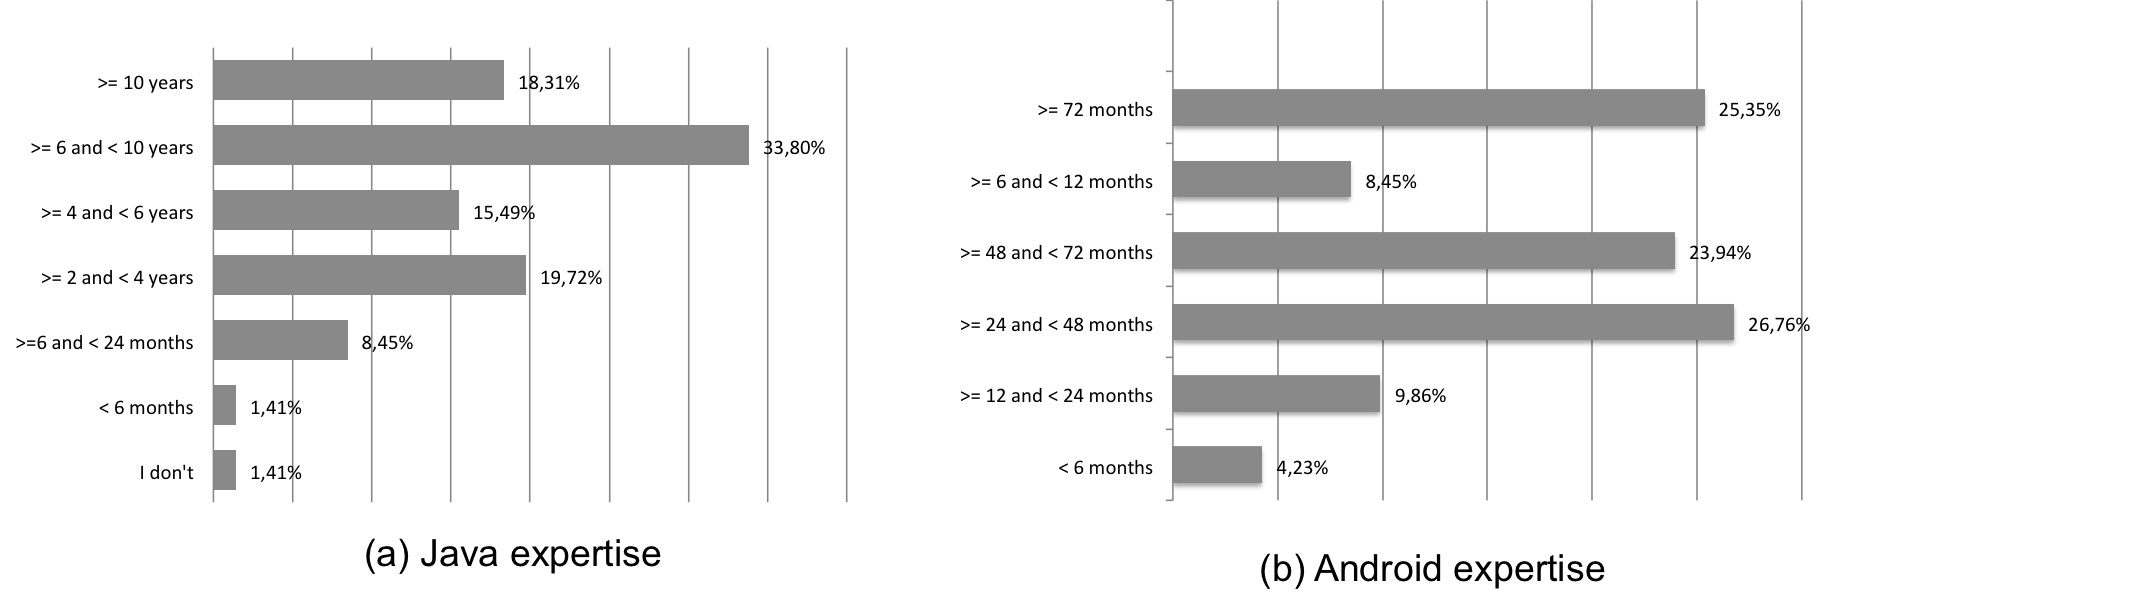
\includegraphics[scale=0.38]{charts/expertise.png}
\caption{Developers expertise in Java and Android development.}
\label{fig:devexpertise}
\end{figure}

\subsection{Findings}

In this section, we present our findings per research question. 
We also include a selection of quotes from the exploratory survey 
respondents. Each respondent has an identification which can be traced in our database. 

\bigskip
\noindent\emph{\textbf{Q1:How developers deal with the exception handling in Android development?}}
\bigskip

This first research question explores the ways in which developers deal with the exception handling code, either throwing or handling exceptions,  while developing an Android app.  Developers were asked about the frequency they develop exception handling code and whether or not they adopt best practices while developing.

%\noindent\emph{Frequency}

Developers were firstly asked how often they dealt with the exception handling code. Many of our survey respondents recognized they have to handle exceptions most of the time during Android app development (64.8\%). However, the frequency on which they throw exception inside apps is smaller; most of the survey respondents said they throw exceptions only some of the time or seldom (80.3\%). It shows that although we can try to avoid dealing with exceptions throwing few exceptions, it is almost always inevitable to handle the exceptions thrown by Android platform and reused libraries. 

\begin{figure} \centering 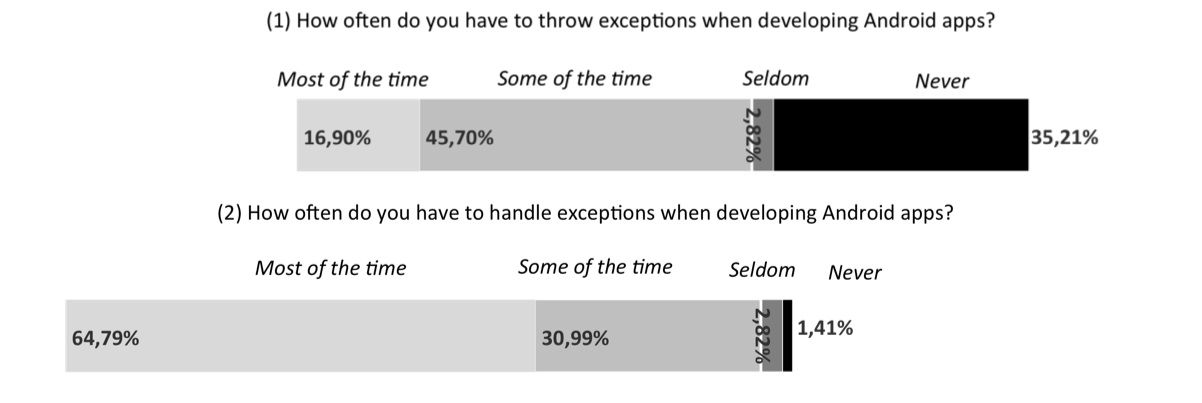
\includegraphics[scale=0.60]{charts/agree_new2.png}
\caption{How often developers throw and handle exceptions during app development.}
\label{fig:oftenhandle}
\end{figure}


\begin{figure} \centering 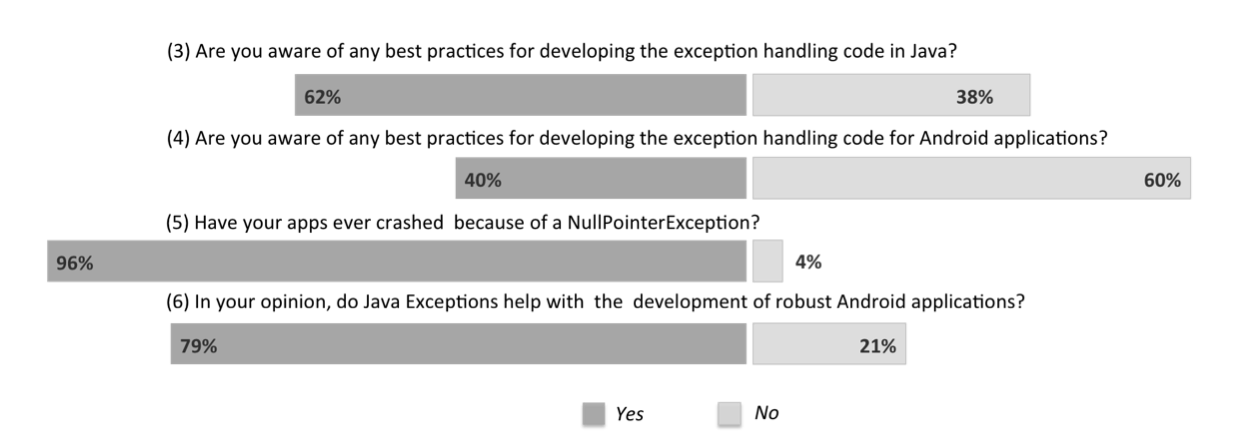
\includegraphics[scale=0.60]{charts/yes_no_new2.png}
\caption{Summary of some survey question answers. }
\label{fig:oftenhandle}
\end{figure}

\bigskip

%\emph{EH Best Practices}
%/////// JAVA BEST PRACTICES ////// 
As mentioned before several general guidelines have been proposed on how to
use Java exceptions. Section XXXXX compiled a list some exception handling (EH) best practices that guided our mining study. In this survey the developers were also asked if they knew about and used Java EH best practices. Although most of them said that knew and adopted Java EH practices 68\%, from this set the most mentioned best practices are presented on Table XXXX - considering that one developer mentioned more than one practice. Some of the practices mentioned, however, are not well known Java EH best practices but seam to be used by some Android developers to better deal with exceptions in Android app context: the crash fast approach [ref], the use of crash report tools, and to favor checked exceptions instead of runtime to represent the exceptional conditions in Android apps.				
	
\begin{table}
\scriptsize
\centering
\begin{tabular}{lrr}
\hline
\bfseries{Top Java EH Best Practices} & \bfseries{\#} & \bfseries{\%} \\
\hline
Use specific handlers / dont catch generic exceptions	& 9 & 23\% \\
Don't swallow Exceptions	 & 7 & 18\% \\
Dont throw Runtime / Favor Checked exceptions & 4 &	10\% \\
Do not use exception for normal  flow control. &	4 &	10\% \\
Free Resources in finally-blocks	& 4	& 10\% \\
crash fast	 & 3 &	8\% \\
crash report tools	&  2 &	5\% \\
Don't catch Errors 	&  2 &	5\% \\
\hline
\end{tabular}
\caption{Top mentioned Java EH best practices -  40 non-empty answers. }
\label{tab:javapractices}
\end{table}			
				
%/////// ANDROID EH BEST PRACTICES /////
The developers who informed that adopted EH best practices were also asked whether they knew about any EH best practice specific to Android context. Most of them 43\% mentioned that they applied the same best practices that they used in Java programs. Only some of them mentioned that adopted specific best practices such as: (i) the use of crash report tools (21\%)  - to notify the developer about the uncaught exceptions that hapen in the application code; and (ii) the use of a global exception handler (14\%) - the UncaughtExceptionHandler advised on Android tutorials [ref].					
					
					
\begin{table}
\scriptsize
\centering
\begin{tabular}{lrr}
\hline
\bfseries{Top Android EH Best Practices } & \bfseries{\#} & \bfseries{\%} \\
\hline
Same as java	& 6 &	43\% \\
Crash report tools	 & 3 &	21\% \\
Add a global exception handler (UncaughtExceptionHandler)	 & 2 & 14\% \\
Use checked exceptions	& 1 &	7\% \\
Use appropriate exception messages	& 1 &	7\% \\
\hline
\end{tabular}
\caption{Top mentioned Android-specific EH best practices -  14 non-empty responses. }
\label{tab:androidpractices}
\end{table}			

\bigskip


\noindent\emph{\textbf{Q 2: How the NullPointerExceptions impact the development of robust Android apps?}}

\bigskip 

%//////NULLPONTER WORSE IN ANDROID /////
Developers were asked if their apps ever crashed  because of a NullPointerException. The vast majority of respondents (96\%) said that their apps crashed at least once due to a NullPointerException. 
Their answers are aligned with the high prevalence of NullPointerExceptions found in the mining study - in Table XXX we can see that NullPointerExceptions were the main cause of the mined exception stack traces.
The developers were also asked whether or not craches caused by NullPointerException were most common in Android development than in stantard Java development.  Almost half of them (XXX\%) mentioned that Android apps were more suceptible to NullPointerException crashes. Some of the reasons mentioned by developers were: (i) the activity and fragment lifecycle - since both are constantly distroyed its references can frequently become null leading to NullPointerExceptions; (ii) the framework complexity - several methods od Android framework return null, and there is not enought documentation to inform the developer when using such methods. 

\greybox{They can happen pretty much anywhere.	 The Android Fragment system comes to mind in this case. Often, it is possible to find yourself in a state where getActivity() is null within the Fragment during certain points in the life cycle, and that is something I have to plan for. This might have been avoidable under a different structure.}


\greybox{The Android framework is what adds the complexity in figuring out what caused an exception because more often than not, the error is triggered from the framework as a result of something else you did.}

Moreover, few respondents also answered that such NullPointerException crashes can be caused by backward compatibility as well as memory issues as illustrated in Table XXXX. The other half mentoned that NullPointerExceptions are  common in Android development as it is common in Java standard development.		
	
\greybox{Honestly, there are a lot of very unskilled Java programmers out there writing Android apps. When they encounter NPE, they tend to null-check that variable, which just puts a bandage on the problem and causes other failures (usually also NPE's) later on in the application's lifecycle.}

%\greybox{This is nothing specific to Android, it's just how Java works.}


\begin{table}
\scriptsize
\centering
\begin{tabular}{lrr}
\hline
\bfseries{Top Ways} & \bfseries{\#} & \bfseries{\%} \\
\hline
activity/fragment life cycle  &	9 &	47\% \\
framework complexity	& 6 &	32\% \\
API / Backward compatibility	& 2 &	11\% \\
memory issues & 	1 &	5\% \\
no layers to catch runtimeexceptions	& 1 &	5\% \\
\hline
\end{tabular}
\caption{Top reasons why NullPointerExceptions are more frequent in Android apps acording to 19 respondents . }
\label{tab:handlingruntime}
\end{table}

%////// PREVENT NULL POINTER /////
Developers were also asked about what they usually do to prevent NullPointerExceptions to happen when their app is in production. Most of them sais that include null-checks on the application code (59\%) mostly when checking the return of a method and as method guard conditions. Many respondents (39\%) also answered that instead of just sprinkling the code with null-checks when a NullPointerException happens they investigate the cause of the null reference and work to fix it, instead of just adding a null check. Some respondents also mention that use annotations such as @Nullable @NonNull, provided in Android since version XXX; such annotations guide de developer about what can and cannot be null during the application lifecycle. Altough catching the NullPointerExceptions is considered a bad practice some respondents said that they do it to prevent crashes caused by NullPointerExceptions. Such behavior was mentioned by one of the responded as the behavior adopted as as way non-expericente developers take to prevent such crashes - which is undoubtly a mistake. Some respondents also mentioned to replace the NullPointerException by IllegalArgumentException when a method should not receive a null as parameter. This is a good exception handling practice mentioned by Bloch in [ref]. Only few developers mentioned about coding standards and static code analyzers to prevent it (2\%).


\greybox{Determine why the object was null and attempt to fix this situation. In the case of external API calls which return null, then check for null (the quick-and-dirty way). For internal calls, use @NotNull and @Nullable annotations to provided more guidance on when an object \"may be\" and \"should never be\" null.}

\greybox{Probably the most common exception, as such the reasons and fixes are super varying. But in general, null checks should be utilized and illegal state or argument exceptions should be used with an appropriate message. Which will communicate useful information without the confusion an NPE would normally cause.}



\begin{table}
\scriptsize
\centering
\begin{tabular}{lrr}
\hline
\bfseries{Top Ways} & \bfseries{\#} & \bfseries{\%} \\
\hline
null-checks &	36 &	59\% \\
investigate/fix the cause	& 24 & 	39\% \\
@Nullable @NonNull &	8 &	13\% \\
catch null-pointer (mistake)	& 3 &	5\% \\
initialize/use default variable	& 3 &	5\% \\
new control-flow for null	& 3 &	5\% \\
avoid using nulls / avoid to use methods can throw null	& 2 &	3\% \\
static analisis	& 2 &	3\% \\
automated testing	& 1 &	2\% \\
make sure value is not null	& 1 &	2\% \\
coding standards	& 1 &	2\% \\
guard statements 	& 1 &	2\% \\
handlers in all entry points	& 1 & 	2\% \\
Use ART more than Dalvik	& 1 &	2\% \\
Use IllegalArgument or IllegaState exception instead	& 1 &	2\% \\
Verify the state of activity/fragment	& 1 &	2\% \\
Write code in Scala, without nulls (joke)	& 1 &	2\% \\
\hline
\end{tabular}
\caption{Top ways for preventing NullPointerException in Android apps - 61 non-empty responses. }
\label{tab:handlingruntime}
\end{table}	


\bigskip 

\noindent\emph{\textbf{RQ 3: How Cross-Type Wrappings impact the development of robust Android apps?}}

\bigskip

Some of the best practices are related to the different ways exceptions should be handled according to whether it is a checked and an unchecked exception. When the designer of an API specifies that a method throws a checked exception, it is telling the caller of the API that such exception should be handled.

%///// HANDLING RUNTIME AND CHECKED /////		
To assess developers perspective on whether checked and unchecked exceptions should be handled different inside the app, the developers were presented to two pieces of code: one on which a RuntimeException was caught and another one where an IOException has caught; both in the contexts of Activity life-cycle methods. Then the developers were asked whether or not the way to handle a runtime exception should be different from the way to handle a checked exception. 

This question was motivated by the fact that during the mining study we could identify that many checked exception were just wrapped in a runtime exception and rethrown, as a way to by pass any kind of handling. When asked about of how to deal with a checked exception signaled by a method (invoked in the context of onPause() activity method), most respondents (62.50\%) said that they should add a try-catch block surrounding the method invocation. Also most of the respondents said that to deal with a method that is signaling a runtime exception we should surround such method by a try-catch block (xxxxx\%). However, what developers mentioned as handling actions (what is performed inside the catch clause to deal with the exception) differes in both cases. 

One of the respondents mentioned that when the designer of an API decides to signal a checked exception s/he is telling the developer that the exception should be handled. Hence, some handling actions mentioned for checked exceptions were: (i) retrying the same operation; (ii) involving the user in finding a solution to the exception condition such as opening a pop-up and asking the user to define a new place to save the file (as in the example presented to them involved a IOException been signaled); and also (iii) presenting an error message to the user. 

On the other hand, the most common way of dealing with a runtime exception would be to catch it and present an error message to the user, or swallow the exception. Some developers also mentioned to use a Toast to support this task\footnote{A toast is an Android component that provides simple feedback about an operation in a small popup - http://developer.android.com/guide/topics/ui/notifiers/toasts.html}. Few developers mentioned that the runtime exception should flow upstream so the framework so it could gracefully crash the app. Although there is a long lasting debate about the pros and cons of checked and unchecked exceptions, most Android developers condireded checked exceptions a way od using exceptions that can prevent uncaught exception crashes - since in order to a checked exception to flow upstream and crash the app the developers needs to explicitly do so. 				

\begin{table}
\scriptsize
\centering
\begin{tabular}{lrr}
\hline
\bfseries{Top Ways} & \bfseries{\#} & \bfseries{\%} \\
\hline
Add a try-catch block &	37 &	59\% \\
Present error message	&  14 &	22\% \\
Log the exception	& 12 &	19\% \\
Throw a checked exception	& 12 & 19\% \\
Let it crash / crash fast 	& 6 &	10\% \\
Swallow the exception	& 5 &	8\% \\
Add a throws declaration	& 5 &	8\% \\
Report crash &	3 &	5\% \\
Use Toast & 	3 &	5\% \\
\hline
\end{tabular}
\caption{Top ways of handling runtime exceptions -  63 non-empty responses. }
\label{tab:handlingruntime}
\end{table}		



\begin{table}
\scriptsize
\centering
\begin{tabular}{lrr}
\hline
\bfseries{Top Ways} & \bfseries{\#} & \bfseries{\%} \\
\hline
Add a try-catch block	& 25 &	63\% \\
Present error message	& 7 &	18\% \\
Involve the user in solving	& 5 &	13\% \\
Retry  &	5 &	13\% \\
Investigate the cause &	3 &	8\% \\
Same way as runtime	& 3 &	8\% \\
Add a throws declaration / pass upstream &	2 &	5\% \\
%Swallow	& 1 &	3\% \\
%Toast	 & 1 & 3\% \\
\hline
\end{tabular}
\caption{Top ways of dealing with a checked exception signaled in the context of an Activity method -  40 non-empty responses. }
\label{tab:handlingruntime}
\end{table}		


%/////// CROSS TYPE WRAPPING //////
Hence, developers were presented to a code snipet on which as cross-type wrapping was performed\footnote{This cross-type wrapping was found in several applicarions during the mining study as well as in some classes of Android framework} - as illustrated in Figure X. Then developers were asked whether such cross-type wrapping could affect the application robustness in some way. Table XXXX illustrates the  most mentioned reasons why cross-type wrapping may affect app robustness; 18\% of the respondents mentioned that the app would crash anyway, regardless the exception was wrapped or not. Most of the respondents, however, mentioned disadvantages of such wrapping such as: (i) it impairs proper handling since when wrapping in a general exception we loose information about the exception situation to he handled (24\%); such wrapping treat all exceptions as critical in other words, every exception will remain uncaught and will lead to an app crash; it does not allow the developer to perform a proper handling (e.g. retry) for exception types that are not critical. 		

{\footnotesize
\begin{verbatim}
  @Override
  public void onPause() {
     try {
        ...
      } catch (Exception e) {
            throw new RuntimeException("...", e);
      }
 }
\end{verbatim}
}

\begin{table}
\scriptsize
\centering
\begin{tabular}{lrr}
\hline
\bfseries{Top Reasons Why Cross-Type Wrapping Affect Robustness} & \bfseries{\#} & \bfseries{\%} \\
\hline
impairs proper handling (loses exception information)	& 12 &	24\% \\
uncaught will crash the app	& 12 &	24\% \\
app will crash anyway	& 9	& 18\% \\
should catch / handle properly (do local recovery)	 & 5 & 	10\% \\
treat all exceptions as critical	& 5 &	10\% \\
useless rethrow	& 2 &	4\% \\
activity mehtods cannot throw exceptions &	1 &	2\% \\

\hline
\end{tabular}
\caption{Top reasons why cross-type wrapping may affect app robustness - 49 non-empty responses. }
\label{tab:handlingruntime}
\end{table}

\bigskip
\noindent\emph{\textbf{RQ 4: Are developers aware of the robustness threats caused by JNI undocumented checked exceptions?}}
\bigskip

%//////// JNI /////
The respondents were presented to a piece of code on which a non-declared checked exception has scaped, and were asked if they new any reason for it to happen. Only 3 respondents out of 71 (4\% of respondents) were aware of the fact that there are ways a method can throw a non-declared checked exception, such as JNI/native code, relfection, and directly changing the bytecode/dalvik code which bypass the compile-time checking.  Most of the repondents were not aware that a method could throw a checked exception withou declaring it on the method's signature. Most respondents mentioned that if a method throws a non-declared exception it must be a RuntimeException. We could observe that this exception handling bug hazard detected during the mining study, although represent a threat to app robustness, is hardly known by the Android developers involved in this survey. Below we can find a quote from one of the 3 respondents aware of JNI non-delcared checked exceptions.

\greybox{I am guessing this is because the exception is thrown from native code (ie, C++ code in the JVM) where Java correct-ness semantics rules do not always apply.}


%\noindent\emph{\textbf{Q2: Do developers know about exception handling best practices?}}
%We can observe that 62\% of surveyed Android developers follow Java exception handling best 
%practices. Among the best practices cited by developers the most popular ones were: avoid generic 
%catches and avoid empty catch blocks. They did not mention a any guide or reference of best practices. 
%When asked about best practices specific to Android developers, most of the developers mentioned that 
%they did no about them. The ones who answered positively said that they adopt the same best practices 
%as in any Java program. 



\noindent\emph{\textbf{RQ5: How the exception handling code affect the development of robust apps and how developers prevent apps from crashing?}}

\bigskip

Developers were also asked whether the exception handling code helped with the development of robust Android applications. Although most of the developers answered positively (78.9\%) when asked to provide one or more reasons for their answers, most of the respondents also provide reasons why the exception handling code can sometimes impairs the robustness.  Since positive and negative reasons were provided intermixed we analyzed both set of answers and ranked the top reasons why exception handling that can negatively or positively affect robustness according to developers perceptions. Table ~\ref{tab:topreasons} presents the top reasons why the exception handling code may or may not help de development of robust apps. 

\begin{table}
\scriptsize
\centering
\begin{tabular}{lrr}
\hline
\bfseries{Top Reasons} & \bfseries{\#} & \bfseries{\%} \\
\hline
\bfseries{For Positively Affecting Robustness} &   &   \\
Improves error diagnosis  &	10	& 15\% \\
Anticipated erroneous situation help writing more robust code  & 9	 & 13\% \\ 
%Anticipated erroneous situation help writing more robust code 
Exceptions only for unrecoverable behavior	& 7 &	10\% \\
Checked exceptions force handling  &	6	& 9\% \\
Useful to gracefully crash 	& 4 &	6\% \\
		
\bfseries{For Negatively Affecting Robustness} &   &   \\
Every exception should be caught to improve robustness	& 7	& 10\% \\
Makes debugging harder &	2 &	3\% \\
Unchecked/runtime exceptions can crash apps & 2	& 3\% \\
NullPointerExceptoins can happen anywhere/are tricky to avoid	 & 2	& 3\% \\
VM inefficiency 	& 1 & 1\% \\

\hline
\end{tabular}
\caption{Top 5 reasons why exception handling helps or impairs the development of robust apps}
\label{tab:topreasons}
\end{table}


Although most of the respondents answered that exception handling code helped with the development of robust Android applications, almost every respondent pointed a drawback associated to he exception handling code, saying that if not used with care the exception handling code may lead to app crashes.  

\greybox{Any uncatched exception will crash the app. There are many unknown exception thrown by the system, that are only happen once in a lifetime like IllegalStateException: eglMakeCurrent failed EGL\_BAD\_CONTEXT}

\greybox{The lifecycle of activities\/fragements etc make it harder to work out what order things are called in and so exceptions can occur because you didn't realise that another method isn't called.}

%\bigskip

Developers were asked to rank the main causes of crashes. Approximately 68\% of the repondents ranked the exceptions signaled by programming logic mistakes e.g. NullPointerExceptions as the Top 1 and Top 2 cause of crashes as illustrated in Figure ~\ref{figure:ranking}. In our mining study the exceptions signaled due to programming logic mistakes (java.lang and util) where the causes of 52,0\% of the exception stack traces found. Hence, the developers perspective is aligned with what was revealed in mining study.
%[width=.9\hsize]
\begin{figure*} 
\centering 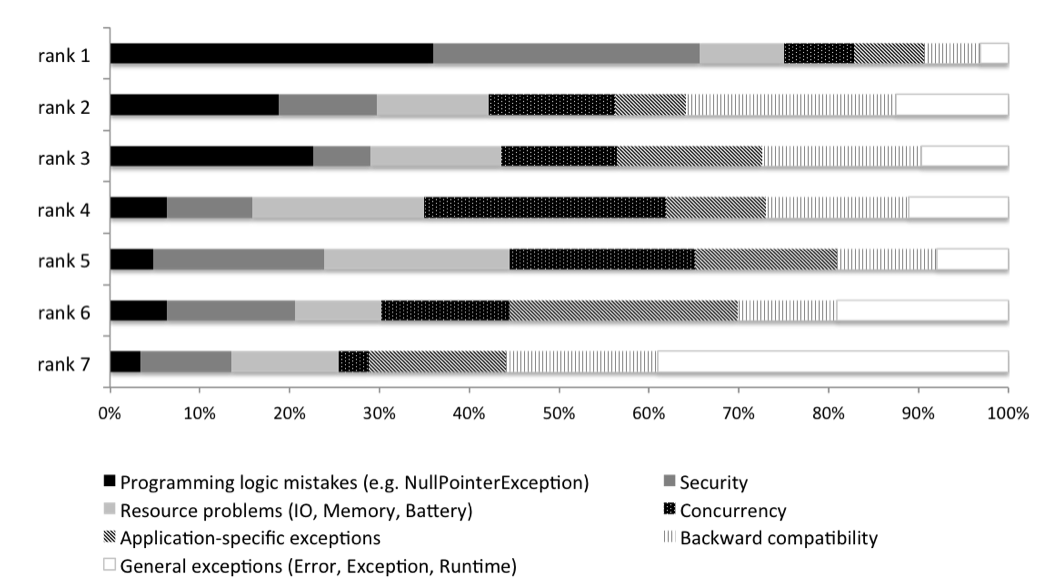
\includegraphics[scale=0.60]{charts/ranking.png}
\caption{Developers perspectives on the main causes of crashes.}\label{fig:ranking} 
\end{figure*}


Finally developers were asked how they prevent their apps from crashing. Most of the respondents answered that they prevent apps from crashing by handling exceptions/errors (27\%). They mentioned about some strategies such as: handling exceptions in all entry points/all over; using catch-all clauses; and adding try catch blocks around risky methods. Different from conventional Java programs, an Android app is composed by several entry points, each window (i.e. Activity) is a potential entry point on which exceptions can scape leading to an app crash. Hence the importance of handling exceptions in all entry points, and using general cash clauses which cannot sometimes prevent crash but allows the developer to present a detailed error message to the user before crashing. Many respondents also said that they used testing approaches to prevent crashes -  few of them mentioned crowd testing (3\%) an emerging approach in testing apps. Moreover, null checks were also mentioned by 15\% of the developers as a way to prevent crashes. The adoption of coding styles were also pointed out by 14\% of respondents as a way to prevent craches. Finally, the crash report tools (e.g. ACRA [ref]) were reported as a way to prevent crashes. Once such tools notify developers about current crashes, the application can be fixed and hence future crashes (caused by what was fixed) could be prevented. Table ~ref{tab:topprevent} presents the themes for the strategies for crash prevention mentioned by developers.	 					
			

\greybox{Though not particular to Android, most Android apps have several different entry points: Activities, Services, etc, can be started by different services; same thing with events. It may be hard to ensure that all this cases are properly handled. }


\greybox{You can wrap the main function in java in try/catch in android you can\'t. }
			
						
\begin{table}
\scriptsize
\centering
\begin{tabular}{lrr}
\hline
\bfseries{Top Ways of Crash Prevention} & \bfseries{\#} & \bfseries{\%} \\
\hline
handling exception/error  & 19 &	27\% \\
testing &	14 &	20\% \\
null check(s) &	11 &	15\% \\
- null check annotations (@Null and @NonNull)	& 3 & 	4\% \\
coding style(s)	& 10 &	14\% \\
crash report / crash report tools &	8	& 11\% \\
\hline
\end{tabular}
\caption{Top ways of preventing crashes - 71 non-empty respondents. }
\label{tab:topprevent}
\end{table}

\bigskip 


\section{Replication Package}
All the data used in the mining study and in the survey-based study is publicly available at the ExceptionMiner tool website hosted in GitHub\footnote{ https://github.com/souzacoelho/exceptionminer}.
Specifically we provide: (i) all issues related to Android projects found
in GiTHub and Google Code used in this study; (ii) all stack traces extracted
from issues; (iii) the results of manual inspection steps; (iv) the
ExceptionMiner tool we developed to support stack trace extraction and distilling; (v) the survey questions; and (iv) the survey responses and summary.

\section{Discussion}
\label{sec:disc}

\begin{quotation}
\noindent
 \emph{``Everybody hates thinking about exceptions, because they are not supposed to happen'' 
  (Brian Foote)}\footnote{Brian Foote shared his opinion in a conversation with James Noble - quoted on the paper: hillside.net/plop/2008/papers/ACMVersions/coelho.pdf}
\end{quotation}

%\emph{\textbf{The exception handling confusion problem.}}

\subsection{The exception handling confusion problem}
When (mis)applied, exception wrapping can make the exception-related code
 more complex and lead to what we call the \emph{exception handling confusion problem}.
This problem can lead the program to an unpredictable state in the presence of exceptions,
as illustrated by the scenario in which a checked exception wraps an OutOfMemoryError. 
Currently there is no way of enforcing Java exception type conventions during program development.
Hence, further investigation is needed on finding ways to help developers in dealing with this
 problem, either preventing odd wrappings or enabling the developer to
 better deal with them.
Furthermore, only some of the Android developers surveyed in this study were aware of the 
rebustness threats caused by cross-type wrappings as the one cited above. This calls for empirical studies on the actual usefulness of Java's hybrid exception model. 

%The cross-type wrappings detected in this study points to the fact that: (1) exception 
%wrappings may prevent exception types from being used according to its initial purpose
%(e.g, Errors should represent situations that should not be handled); and (2) may have been
% used to bypass the language restrictions imposed by checked exceptions  (e.g,
% checked exceptions may be wrapped in runtime exceptions).

%\emph{\textbf{On the null pointer problem.}}
\subsection{On the null pointer problem.}
The null reference was firstly introduced by Tony Hoare in ALGOL W, which after some years he called his ``one-billion-dollar mistake''~\cite{hoare2}.
In this sudy, the null references were, infact, responsible for several reported issues - providing further evidence to Hoare's statement. Moreover many of the survey respondents recognized that NullPointerExceptions was one of the main causes of application crashes since they can happen almost 
anyware in the application code, and to make thinks worse the life-cycle of Android apps on which objects are constantly recreated (i.e., Activity and Fragment classes) favor this kind of exception to happen added to the fact that many Android framework methods return null without making such
return type explicitly on the documentation.
Such observations emphasizes the need for solutions to avoid NullPointerExceptions, such as:
(i) lightweight intra-method null pointer analysis as supported by
Java 8 @Nullable annotations\footnote{Already supported by tools such as Eclipse, IntelliJ, Android Studio 0.5.5 (release Apr. 2014) to detect potential 
null pointer dereferences at compile time.};
(ii) inter-method null pointer analysis tools such as the one proposed by Nanda and Sinha~\cite{nanda2009accurate};
or (iii) language designs which avoid null pointers, such 
as Monads~\cite{Walde95} (as used in functional languages for values that may not be available 
or computations that may fail) could improve the robustness of Java programs. 
Some of the Android developers mentioned how @Nullable annotations could helpful to deal with
NullPointerExceptions and consequently prevent app crashes caused by it.


%\emph{\textbf{Preventing uncaught exceptions}}
\subsection{Preventing uncaught exceptions}
In this study we could observe undocumented runtime exceptions thrown by third party code,
and even undocumented checked exception thrown by a JNI interface.
Such undocumented exceptions make it difficult, and most of the times infeasible
for the client code to protect against `unforeseen'' situations that may happen 
while calling a library code. In the survey-based study Android developers were asked about
ways to prevent application crashes which are mainly caused by uncaught exceptions.
Many of them emphasized the importance of handling exceptions to prevent crashes
but also mentioned how difficult is to handle every specific exception that can happen.
Several developers recognized to follow a more reactive behaviour against crashes:
they advocate the use of crash report tools, and once the crash happens for the first time,
its reported and the application can be changed to better cope with the exceptions that crashed the crashes, consequently preventing future similar crashes.

One may think that the solution for the uncaught exceptions may be to define a general handler, 
which is responsible for handling any exception that is not
adequately handled inside the applications. Although this 
solution may prevent  the system from abruptly crashing, as mentioned by some of the surveyed developers such a general handler will not have enough
contextual information to adequately handle the exception, 
beyond storing a message in a log file and restarting the application.
However, such a handler cannot replace a carefully designed exception 
handling policy~\cite{Robil00}, which requires
third-party documentation on the exceptions that
may the thrown by APIs used. 
Since  documenting runtime exceptions is a tedious and error prone
task, this calls for tool support to automate the extraction of runtime exceptions
from library code. Initial steps in this direction have been proposed
by van Doorn and Steegmans \cite{van2005combining}.



%\section{Threats to Validity}
%\label{sec:threats}
%\noindent

%\emph{\textbf{Threats to Validity of the Mining Study.}} 
\subsection{Mining Study - Threats to Validity }

\emph{Internal Validity.} We used a heuristics-based parser to mine
exceptions from issues.  Our parsing strategy was conservative by default; for
example, we only considered exception names using a fully qualified class name
as valid exception identifiers, while, in many cases, developers use the
exception name in issue description. Conservative parsing may minimize false
positives, which was our initial target, but also tends to increase false
negatives, which means that some cases may have not been identified as
exceptions or stack traces. Our limited manual inspection did not reveal such
cases. Moreover, in this study we manually mapped the concerns related
to exceptions. To ensure the quality of the analysis, we calculated the
 interrater agreement after three independent 
developers classified a randomly selected sample (of 25 exception 
types from the total of 100); the interater agreement was high (96\%). 

\emph{External Validity.} Our work uses the GHTorrent dataset, which although 
comprehensive and extensive is not an exact replica of Github. 
However, the result of this study does not depend on the analysis of
a complete Github dataset. Instead, the goal of our study was to 
pinpoint \emph{bug hazards} on the exception-related code based on 
exception stack trace mining of a subset of projects.
We limited our analysis to a subset of existing open-source Android projects.
We are aware that the exception stack traces reported 
for commercial apps can be different from the ones found in this study, and that
this subset is a small percentage of existing apps.
Such threats are similar to the ones imposed to other empirical studies 
which also use free or open-source Android apps~\cite{Linar13,McDon13,Ruiz12}.
Moreover, several exception stack traces that support the findings of this study
refered to exceptions coming from methods defined on Android Application Framework
and third-party libraries.  Additionaly,  the \emph{bug hazards} observed in this study are due to
characteristics of the Java exception model, which can impose challenges 
the robustness of not only to Android apps but also to other systems
 based on the same exception model. 

Another threat relates to the fact that parts of our analysis 
are based on the availability of stack traces on issues reported on Github and Googlecode projects. 
In using these datasets, we make an underlying assumption: the stack traces reported on issues are 
representative of valid crash information of the applications. 
One way to mitigate this threat would be to access to the full 
set of crash data per application. Although some services exist 
to collect crash data from mobile applications~\cite{BugSe14,BugSn14,Googl14,Acra14},
they do not provide open access to the crash reports of their client applications.
In our study, we mitigated this threat by manually inspecting
the source code associated to a subset of the reported exception stack traces.
This subset comprises the stack traces related to the main findings 
of the study (e.g., ``undocumented runtime and checked exceptions'',
and ``cross-type wrappings'').

\subsection{Limitations of the Survey-based Study.}
Due to the exploratory nature of the second phase of this work whose 
goal was to identify the developers perspectives concerning the exception 
handling bug hazards found during the repository mining 
phase, we choose Gounded Theory techniques. The results of our
survey-based study may not apply to every Android developer, since other populations 
might add new insights.  The population we collected data from was comprised 
by Android developers of the GitHub 
Android projects whose issues were mined on the first phase of this work, and who had
time and motivation to answer the survey questions.

Altough the themes and findings that emerged in our study cannot 
be generalized, they give a first view of developers perspectives about
 EH bug hazards found. Hence, we believe that the survey-based study 
have contributed with valuable insights about how Android developers 
used the exception handling code and what are their perspectives regarding
exception handling bug hazards.



%\noindent




\section{Related Work}
\label{sec:rele}

In this section, we present work that is related to the present paper, divided into
four categories as detailed next.

\textit{Analysis and Use of Stack Trace Information.} Several papers have
investigated the use of stack trace information to support: bug classification
and clustering~\cite{wang2013improving, kim2011crash, dhaliwal2011classifying},
fault prediction models~\cite{kim2013predicting}, automated
bug fixing tools~\cite{sinha2009fault} and also the analysis of Android APIs~\cite{kechagia2014}. 
Kim et al.~\cite{kim2011crash} use an
aggregated form of multiple stack traces available in crash reports to detect
duplicate crash reports and to predict if a given crash will be fixed. Dhaliwal
et al.~\cite{dhaliwal2011classifying} proposed a crash grouping approach that
can reduce bug fixing time in approximately 5\%. Wang et
al.~\cite{wang2013improving} propose an approach to identify correlated crash
types and describe a fault localization method to locate and rank files related
to the bug described on a stack trace. Schroter et al.~\cite{schroter2010stack}
conducted an empirical study on the usefulness of stack traces for bug fixing
and showed that developers fixed the bugs faster when failing stack traces were
included on bug issues.  In a similar study, Bettenburg et
al.~\cite{bettenburg2008makes} identify stack traces as the second most stack
trace feature for developers.  Sinha et al.~\cite{sinha2009fault} proposed an
approach that uses stack traces to guide a dataflow analysis for locating and
repairing faults that are caused by the implicitly signaled exceptions. Kim
at al.~\cite{kim2013predicting} proposed an approach to predict the
crash-proneness of methods based information extracted from stack traces and
methods' bytecode operations.  They observed that most of the stack traces were
related to NullPointerException and other implicitly thrown exceptions had
the higher prevalence on the analyzed set of stacks. Kechagia and Spinellis~\cite{kechagia2014}
examined the stack traces embedded on crash reports sent by 1,800 Android apps 
to a crash report management service (i.e., BugSense). They found that 19\% of such stack traces
were caused by unchecked and undocumented exceptions thrown by methods defined on 
Android API (level 15). Our work differs from Kechagia and Spinellis since it is based on
stack traces mined from issues reported by open source developers on GitHub and Googlecode.  
Moreover, our study mapped the origin of each exception 
(i.e., libraries, the Android platform or the application itself) and investigated
the adoption of best practices based on the analysis of stack trace information.
Our work also identified the type of each exception mined from issues
(classifying them as Error, Runtime or Checked) based on the source code
analysis of the exception hierarchy and analized the exception wrappings that can 
happen during the exception propagation.  Such analysis revealed intriging 
\emph{bug hazards} such as the cross-type exception wrappings not discussed in previous works.


\textit{Extracting Stack Traces from natural language artifacts.} 
Apart from issues and bug reports, stack traces can be embedded in other forms of
communication between developers, such as discussion logs and emails.
Few tools have been proposed to mine stack traces embedded on such resources.
 Infozilla~\cite{bettenburg2008extracting} is based on a set of regular expressions that extract a set of frames
related to a stack trace. The main limitation of this solution is that it is not
able to extract stack traces embedded on verbose log files (i.e., on which we
can find log text mixed with exception frames). Bacchelli
et al.~\cite{bacchelli2012content} propose a solution to recognize stack trace frames
from development emails and relate it to code artifacts (i.e. classes) mentioned
on the stack trace. In addition to those tools, ExceptionMiner is able to 
both extract stack traces from natural language artifacts and to 
classify them in a set of predefined categories.

\textit{Empirical Studies on Exception Handling Defects.} 
Cabral and Marques~\cite{cabral2007exception} analyzed the
source code of 32 open-source systems, both for Java and .NET. They
observed that the actions inside handlers were very simple (e.g., logging and present a
message to the user). Coelho et al.~\cite{coelho2008assessing} performed an 
empirical study considering the fault-proneness of aspect-oriented implementations 
for handling exceptions. Two releases of both Java and AspectJ implementations were 
assessed as part of that study. Based on the use of an exception
flow analysis tool, the study revealed that the AOP  refactoring increased the 
number of uncaught exceptions, degrading the robustness of the AO version of every analyzed system.
The main limitation of approaches based on static analysis based approaches are the number of false
positives they can generate, and the problems the faced when dealing with reflection libraries 
and dynamic class loading. Pingyu and Elbaum~\cite{Zhang12} were the first to perform
an empirical investigation of issues, related to exception-related bugs, on Android projects.  
They perform a small scale study on which they manually inspected the issues of 
5 Android applications. They observed that 29\% had to do with poor
exceptional handling code, this empirical study was used to motivate the development of a tool
aiming at amplifying existing tests to validate exception 
handling code associated with external resources. This work inspired ours,
 which automaticaly mined the exception stack traces embedded on issues 
reported on 639 open source Android projects. The goal of our study was
to identify common \emph{bug hazards} on the exception related code that can lead to 
failures such as uncaught exceptions. 

\textit{Empirical studies using Android apps.} Ruiz et al.~\cite{Ruiz12}
investigated the degree of reuse across applications in Android Market, the
study showed that almost 23\% of the classes inherited from a base class in the
Android API, and that 217 mobile apps were reused completely by another mobile
app. Pathak et al.~\cite{Patha11} analyzed bug reports and developers
discussions of Android platform and found out that approximately 20\% of
energy-related bugs in Android occurred after an OS update. McDonnell et
al.~\cite{McDon13} conducted a case study of the co-evolution behavior of
Android API and 10 dependent applications using the version history data found
in GitHub. The study found that approximately 25\% of all methods in the client
code used the Android API, and that the methods reusing fast-evolving APIs were
more defect prone then others. Vasquez et al.~\cite{Linar13} analyzed
approximately 7K free Android apps and observed that the last successful apps
used Android APIs that were on average 300\% more change-prone than the APIs
used by the most successful apps. Our work differs from the others as it aims at
distilling stack trace information of bug reports and combine such information
with bytecode analysis, source code analysis and manual inspections
to identify \emph{bug hazards} on the exception handling code of Android apps.


\textit{Exploratory Survey Studies.} Exploratory surveys have been used in the software
engineering context to discover the user perspective regarding a broad range of 
topics such as: how developers define productivity [ref]; how GitHub developers use
pull-requests[ref]; how the testing culture of open-shource projects can be characterized [ref]; 
and even how developers use Twiter [ref]. This kind of study is important as a way of 
better understanding the developers behavior and hence provide recommendations and 
tools to help on specific development tasks. This was the first exploratory survey study whose
goal was to assess developers perspective regarding a set of exception handling bug hazards
as well as how developers deal with exceptions and prevent crashes while developing.
 



%\enlargethispage{-2\baselineskip}

\section{Conclusion}
\label{sec:conc}

The goal of this paper is two-fold: (i) to investigate 
to what extent stack trace information can reveal \emph{bug hazards} 
related to exception handling code that may lead to a decrease in
application robustness; and (ii) to assess the developers perspective
concerning the detected EH \emph{bug hazards}. 

To that end, we mined the stack 
traces embedded in all issues defined in 482 Android projects hosted in Github and 
157 projects hosted in Google Code - overall it included 6,005
exception stack traces. And we surveyed developers associated to some of 
the mined GitHub projects.
Our first key contribution is
a novel approach and toolset (ExceptionMiner) for analyzing Java
  exception stack traces as occurring on GitHub and Google Code
  issues.
Our second contribution is
an empirical study of over 6000 actual stack traces,
  demonstrating that (1) half of the system crashes are due to errors
  in programming logic, with null pointer exceptions being most
  prominent;
  (2) Documentation for explicitly thrown RuntimeExceptions is almost
  never provided; 
  (3) Extensive use of wrapping leads to hard to understand chains
  violating Java's exception handling principles.
Our third contribution was the first exploratory to assess the 
developers perspective concerning the exception handling 
bug hazards in Android development.
 Our results shed light on common problems and bug hazards in Java
exception handling code, and call for tool support to help developers
understand their own and third party exception handling and wrapping logic.

%\begin{acknowledgements}
%If you'd like to thank anyone, place your comments here
%and remove the percent signs.
%\end{acknowledgements}

% BibTeX users please use one of
\bibliographystyle{spbasic}      % basic style, author-year citations
\bibliography{android-stacks}   % name your BibTeX data base


\end{document}
% end of file template.tex

